
\mychapter{Introduction}

\thispagestyle{empty}
\frenchspacing

\section{Śivadharma corpus}
\fancyhead[CE]{{\footnotesize \textit{Vṛṣasārasaṃgraha}}}
\fancyhead[CO]{{\footnotesize \textit{Introduction}}}
\fancyhead[LE]{}
\fancyhead[RE]{}
\fancyhead[LO]{}
\fancyhead[RO]{}

%start of checking with CGPT
The \Vss\ is a 24-chapter-long Sanskrit Śaiva text of the 
so-called \Sivadharmacorpus.  We have no evidence that it
was ever transmitted independently of this collection of texts,%
		\footnote{For cases that may seem exceptions 
		(\msKoa\ and \msPaperA\ \CHECK\ if more)
                see the manuscript descriptions
                on pp.~\pageref{mss_descr}ff.}
			% As already remarked in \mycitep{KissVolume2021}{185, n.~9}, 
                        % MS G 4076 at the Asiatic Society, Calcutta, while seemingly an independent MS}
that has come down to us in multiple-text manuscripts typically containing the following eight works:
\SDhS\ (\SDHS), \SDhU\ (\SDHU), \SDhSangr\ (\SDHSANGR),
\Ums\ (\UMS), \Uums\ (\UUMS), \Vss\ (\VSS), \DharmP\ (\DHARMP), and the \SivaUp\ (\SIVAUP).

Much has now been written on the corpus itself and on the individual texts it comprises. 
For an introduction, an overview of the secondary literature, 
a nearly up-to-date bibliography, and the results of recent research related to the \Sivadharma,
see \mycite{SivadharmamrtaVolume2021}. Important publications that appeared after the release of that volume
include \mycite{HarimotoMunichMS} the Munich MS (MS M), and the formation of the \Sivadharmacorpus,
and \mycite{RitesOfFasting}, which offers a critical edition, translation, and analysis of chapter ten of the 
\SDhS.


Since the \VSS's links to other texts of the corpus---except possibly the 
\DharmP---are relatively weak, I will refer to the Śivadharma corpus and
its texts only when they are relevant for the present inquiry.
%		\footnote{Mainly in section `\CHECK' on p.~\pageref{vss_connection_other_sd_texts}}



\section{Title}\label{title}
The title \Vss%
	\footnote{Read \Vss\ for \titleface{Vṛttasārasaṅgraha}
	in \mycitep{PetechHistory}{84}.}
can be translated as `Compendium on the Essence of the Bull [of Dharma].'
The last two elements (\skt{sāra-saṃgraha}) need
little explanation: this work is a `compendium,' a `collection' or `summary' of (\skt{saṃgraha})
the `essence' (\skt{sāra}), of its topic---that is, a distilled version of relevant teachings.
The words `compendium' and `collection' clearly reflect the composite nature of
the \VSS; see details on the structure of the text and
on its possible sources on pp.~\pageref{structure}ff.

The\label{bull} remaining question is whether the bull in the title 
is only a reference to a representation of Dharma 
or whether it also hints at Śiva's bull, his vehicle or mount,
sometimes called Nandi or Nandin in other works.%
		\footnote{There is no trace of Nandi/Nandin
		as identified with the bull in the \Vss.
		On the possible time after which 
		Nandi or Nandin, originally a \cskt{gaṇa}{gana},
		was considered a \csindex{bull}, see 
		\mycite{bhattacharya_nandin_1977} and 
		\mycitep{Pancavaranastava}{100--108 and 171--172}.}

Dharma is frequently referred to as a bull, 
often depicted as losing a leg in every Kalpa.
This portrayal appears in Dharma literature from at least the time of the \MBh;
see, e.g., \MBH\ 3.188.10--12,%
	\footnote{\skt{kṛte catuṣpāt sakalo nirvyājopādhivarjitaḥ |      \\
	              vṛṣaḥ pratiṣṭhito dharmo manuṣyeṣv abhavat purā || \\
				  adharmapādaviddhas tu tribhir aṃśaiḥ pratiṣṭhitaḥ |\\
				  tretāyāṃ dvāpare 'rdhena vyāmiśro dharma ucyate || \\
				  tribhir aṃśair adharmas tu lokān ākramya tiṣṭhati |\\
   				  caturthāṃśena dharmas tu manuṣyān upatiṣṭhati ||}}
and \Manu\ 1.81a
(\skt{catuṣpāt sakalo dharmaḥ}) and 8.16a
(\skt{vṛṣo hi bhagavān dharma}).%
	 \footnote{See, e.g., \mycite{CoutureDharma}.
	 \citeauthor{GutierrezEmbodiment} (\citeyear{GutierrezEmbodiment})
	 sums up the trope thus
	 (in the section `In animal terms'): 
	 `The emphasis on the whole body, with all four legs, assures 
	 the maintenance of stability in dharma's structure, which in 
	 turn structured Brahmanical society.'}
In addition, in Śaiva contexts, the bull of Dharma
does feature as Śiva's vehicle. See, e.g., Bakker's argument, who,
after analysing seals containing images of bulls, remarks:%
                \footnote{\mycitep{BakkerWorld2014}{69}.}


\begin{quote}
The topicality of the Śaiva accommodation 
of the Dharma in the second half of the 
sixth century is nicely illustrated by a myth found in the
original \titleface{Skandapurāṇa}[; \dots]
the uncontrollable, wild bull \ie{vṛṣa} is 
domesticated by Śiva's Gaṇapa\linebreak Prabhākara [\dots]
In this way the bull is transformed into Śiva’s vehicle \ie{vāhana}. 
\end{quote}

\noindent
To put the same argument more bluntly:

\begin{quote}
Making the bull Śiva's vehicle implies that Śiva has become
the supreme lord of the Dharma, or that the Dharma has 
been accommodated in [Ś]aivism.%
	\footnote{\mycitep{SkandaIIb}{65 n.~210}.
	\citeauthor{bhattacharya_nandin_1977} 		
			(\citeyear{bhattacharya_nandin_1977}, {1552}) 
			suggests that `In the Purāṇas the bull
		(\csindexxx{Vṛṣabha}{vrsabha}{\skt{vṛṣabha}} or 
		\csindexxx{Vṛṣa}{vrsa}{\skt{vṛṣa}}) 
	of Śiva is identified with Dharma, ``virtue personified''. 
		This is a new development to sanctify the animal 
		vehicle of the god. This new situation took place with the 		
		religious rite when an offering of a bull to a Brahmin   
		deemed to be	of a high religious merit.'}
\end{quote}
%\vfill\pagebreak

\noindent
The possibility that the bull in the title \Vss\ refers 
not only to Dharma as a bull, but also
to Śiva's \skt{vāhana} has been mentioned
in\linebreak
\mycite{UmaSivaPlay},%
        \footnote{P. 238 n.~13.}
and briefly discussed in \mycite{KissVolume2021},%
        \footnote{Pp. 185--186.} 
with the conclusion that 

\begin{quote} 
while the bull as a synonym of Dharma is mentioned in the text repeatedly,
somewhat surprisingly, and perhaps significantly, there is no
clear reference to Śiva's mount in the \Vss. [\dots\ Nevertheless, it]
is not inconceivable that the redactors of the \Vss\ had
the same association in mind, namely that the bull in 
question is both Dharma and Śiva's mount.%
	\footnote{Note that \SDhU\  12.87
				also mentions the `Dharma bull':
	    \skt{īśvarā\-yatanasyādhaḥ śrīmān dharmavṛṣaḥ sthitaḥ} |
    	\skt{yatra vīravṛṣas tatra kṣityāṃ gomātaraḥ sthitā} ||. 
                `Below the abode of the Lord, there lives the glorious Dharma Bull.
                 Where the Heroic Bull is in the world, there are the Cow Mothers.'}
\end{quote} 

%Śiva got his bull, MBh:
%13076027a vṛṣabhaṃ ca dadau tasmai saha tābhiḥ prajāpatiḥ
%13076027c prasādayām āsa manas tena rudrasya bhārata
%13076028a prītaś cāpi mahādevaś cakāra vṛṣabhaṃ tadā
%13076028c dhvajaṃ ca vāhanaṃ caiva tasmāt sa vṛṣabhadhvajaḥ
%13076029a tato devair mahādevas tadā paśupatiḥ kṛtaḥ
%13076029c īśvaraḥ sa gavāṃ madhye vṛṣāṅka iti cocyate

%MMW `vṛṣa':\\
%``Justice or Virtue personified as a bull or as''Siva's bull Mn. viii,
%16 Pur. Kāvyād.; just or virtuous act, virtue, moral merit ``Siś.
%Vās.;''

%Mahākṣapaṇaka's koṣa (CHECK date), the Anekārthadhvanimañjarī, places
%the meaning `dharma' as first when defining the word `vṛṣa':
%
%\begin{quote}
%    \skt{dharmo vṛṣo vṛṣaḥ śreṣṭho vṛṣo gaur mūṣiko vṛṣaḥ} |\\
%    \skt{vṛṣo balaṃ vṛṣaḥ kāmo vṛṣalo vṛṣa ucyate} || 1.48
%    \end{quote}

% Śivapurāṇa:
% śuddhasphaṭikasaṃkāśo vṛṣabhaḥ sarvasundaraḥ ||
% yo dharma ucyate vedaiḥ śāstraiḥ siddhamaharṣibhiḥ ||54||
% tam ārūḍho mahādevo vṛṣabhaṃ dharmavatsalaḥ||
% śuśubhe 'tīva devarṣisevitaḥ sakalair vrajan ||55||


%visnusmrḍn:ViS 86.15a/ vṛṣo hi bhagavān dharmaś catuṣ-pādaḥ prakīrtitaḥ
%/
%
%Śivapurāṇa 2.3.40.54--55:
%
%\begin{quote}
%\skt{śuddhasphaṭikasaṃkāśo vṛṣabhaḥ sarvasundaraḥ} |\\
%\skt{yo dharma ucyate vedaiḥ śāstraiḥ siddhamaharṣibhiḥ} ||\\
%\skt{tam ārūḍho mahādevo vṛṣabhaṃ dharmavatsalaḥ} |\\
%\skt{śuśubhe 'tīva devarṣisevitaḥ sakalair vrajan} ||
%\end{quote}
%also quoted by \mycitep{bhattacharya_nandin_1977}{1553}	

%smrti/dharma/krtyaratnaakara.dn: !!! dharmo 'yaṃ vṛṣarūpeṇa nāmnā
%nandīśavaro vibhuḥ \textbar{} dharmān māheśvarān vakṣyaty ataḥ prabhṛti
%nārada\textbar{}\textbar{}
%
%tak2015/AtmapujaT55Muktabodha.dn: dharmas tatra vṛṣākāro jñānaḥ
%siṃhasvarūpakaḥ \textbar{} vairāgyaṃ

%On the title, see 
%\mycite{DeSiminiMSSFromNepal2016} (238, n.\thinspace 13):
% `'As noted by \Sanderson\
%{[}\ldots{}{]}, this title can have a double meaning, since the `bull'
%(vṛṣa) is both a synonym of `religious practice' and the traditional
%mount (vāhana) of Śiva. i.e.~Sanderson (Forthc. b), Śaivism and
%Brahmanism. (can't find it)

\noindent
Sanderson (\citeyear{SandersonTolerance2015}, 210 n.~136) comments
on the idea of \cskt{vṛṣa}{vrsa} being Dharma
in general, and on the bull appearing on the coins of the 
Hephthalite Hun Mihirakula in particular, also referencing the \VSS: 

\begin{quote}
To laud the bull (\cskt{vṛṣa}{vrsa}) 
would be surprising if the intended meaning were 
the bull that is Śiva's mount, but not if the word is intended in its figurative meaning, namely \skt{dharmaḥ}, 
or \skt{su\-kṛtam} `the virtuous actions [prescribed by
the Veda].' For this meaning of \skt{vṛṣaḥ} see, for example,
Amarasiṃha, \skttitle{Nāmaliṅgā\-nuśāsana}{Namalinganusasana} 
1.4.25b (\skt{sukṛtam vṛṣaḥ}),
3.3.220 (\skt{sukṛte vṛṣabhe\linebreak vṛṣaḥ}); 
Halāyudha,
\skttitle{Abhidhānaratnamālā}{Abhidhanaratnamala} 1.125cd (\skt{dharmaḥ puṇyaṃ vṛṣaḥ śreyaḥ
sukṛtaṃ ca samaṃ smṛtam}); 
\Manu\linebreak 8[.]16a
(\skt{vṛṣo hi bhagavān dharmas}\dots); 
and the Gwalior Museum Stone
Inscription of Pataṅgaśambhu (\mycite{MirashiGwalior1962}), l. 15,
\skt{vṛṣaikaniṣṭho `pi jitasmaro 'pi yaḥ śaṅkaro 'bhūd 
bhuvi ko 'py apūrvvaḥ}, 
concerning the Śaiva ascetic Vyomaśambhu: 
`He was in the
world an extraordinary new Śiva, since he too was 
\skt{vṛṣaikaniṣṭhaḥ}
(`devoted solely to pious observance'; 
in Śiva's case `riding only on the Bull') and he too was 
\skt{jitasmaraḥ} (`one who had defeated sensual
urges'; in Śiva's case `the defeater of the Love god Kāmadeva'). 
This is also the meaning of \skt{vṛṣaḥ} in the title \Vss,
one of the works of the Śivadharma corpus 
(see, e.g., \mycitep{SandersonSaivaLit2014}{p.~2}), i.e., 
`Summary of the Essentials of the [Śiva]dharma'. 
\end{quote}

\noindent
In the last sentence, \Sanderson\ implies that the
\VSS\ is organically part of the teachings that we
may collectively call the Śivadharma, and he
thus supplies `Śiva' when translating the title \Vss.
A closer examination of the \VSS\ 
reveals no direct references to either Śiva's bull or
to the bull embodying the Śivadharma. Instead, the bull
in the \VSS\ is repeatedly associated with the Dharma which
is the four \asrama s (see, e.g., \VSS\ 3.1--5 and 4.74).
My conclusion here is that while the word \cskt{vṛṣa}{vrsa} in the
title may indeed refer to Śiva's bull, 
this reference is always only implied and never explicitly stated,
whereas the bull as the personification of Dharma as the four
\asrama s appears explicitly and repeatedly. Thus
the title lacks any explicit hint to Śaivism,%
	\footnote{In contrast, see an explicit equation of the bull
	of Dharma with Śiva's mount in the \UUMS\
					(\msCa\ fol.~184r ll. 3--4; see
					\mycitep{KissVolume2021}{185--186}):
		\skt{īśvara uvāca |
  			na jānanti ca loke 'smin mānavā mūḍhacetasaḥ |
 			catuṣpādo bhaved dharmaḥ śuklo 'yaṃ mama vāhanaḥ ||};
		    `Īśvara spoke: In this world, foolish people do not know that
		    the four-legged Dharma is this bright mount of mine.'}
which aligns well with the text's blurred and multi-layered
affiliation to Dharmaśāstra, Vaiṣṇavism, and Śaivism.%
		 \footnote{See p.~\pageref{structure}.}
%		\footnote{See also \mycitep{BakkerWorld2014}{69}, who 
%			while discussing a seal of Śarvavarman that 
%			features a beautifully carved bull representing Dharma,
%			remarks (italics mine): `The reader \textit{may} also see in the 
%			image the thriving Śaiva religion, represented
%			by the Bull, the vāhana of Śiva [\dots]'} 




%\mysubsubsection{Vṛṣadeva's commission?}{vrsadevas-commission}
Finally, as a fanciful experiment, and if one accepts 
that the \VSS\ originated in Nepal,%
		\footnote{See pp.~\pageref{provenance}ff.}
one could wonder whether the title \Vss\ 
has anything to do with the Licchavi king Vṛṣadeva.
\citeauthor{SandersonSaivaAge} 
(\citeyear{SandersonSaivaAge}, 74) mentions that  
Vṛṣadeva is `described in an inscription of his eighth-century 
descendant Jayadeva as having inclined towards Buddhism;%
                 \footnote{See \mycitep{Vajracarya1973}{148, l. 9}: \skt{sugataśāsanapakṣapātī}.}
\linebreak a view confirmed by a local chronicle, which attributes to
him the establishing of Buddhist images,'
%fn: Lévi 1990, vol. 2, p. 98.
and that this king established 
`the Caitya of the Sı̄nagu-vihāra (the Svayambhūnāth Caitya).'
More importantly,\linebreak Sanderson summarises the 
information found in the Chāṅgu Nārāyaṇa Pillar Inscription (east shaft),%
                \footnote{See, e.g., \mycitep{GnoliNepInscr}{1}, \mycite{RiccardiChangu} and\phantom{\hskip10em}\linebreak 
		https://siddham.network/inscription/in02001/} 
noting that Vṛṣadeva was the great-grand\-father of Mānadeva, whose
`dated inscriptions range in date from 459 to 505/6' [\CE].%
                \footnote{\mycitep{SandersonSaivaAge}{75}.}
%	   \footnote{Vṛṣadeva was succeeded by Śaṅkaradeva and   		            Dharmadeva.}
This would place the reign of Vṛṣadeva around 400 \CE. 

The early fifth century may look too early for the date of composition
of the \VSS, and any connection between this king
and the text is impossible to prove at the moment.
However, it is equally impossible to dismiss it entirely.
If such a connection exists, it might explain the slightly unusual nature of the title (`\dots\ the essence of the bull').
\hide{
%https://siddham.network/inscription/in02087/
%https://siddham.network/inscription/in02087/?section=translation
%https://siddham.network/inscription/in02002/
%https://siddham.network/inscription/in02001/
%https://infogalactic.com/info/Licchavi_(kingdom):
}

%
%Gopālarājavaṃśāvalī p. 124 Dharmadeva and a vṛṣa statue? Text mentions vṛṣadhvaja though...
%
%Pañcāvaraṇastava 71:
%pratyag āśāsthitaṃ vande vṛṣaṃ ca vṛṣabhākṛtim|
%sākṣād dharmaṃ sitaṃ tryakṣaṃ parameśasya vāhanam||
%+ notes to this verse on p. 171






\section{Genre}

Some texts of the Śivadharma corpus have, at certain points in their textual history,
been recognised as Purāṇas or Upapurāṇas (see, e.g., \mycite{HazraSDh} and \citeyear{HazraSDhU}).
Could the \VSS\ be considered a Purāṇa? There are at least two reasons to support this idea.

One is the section spanning \VSS\ 1.62--75, which provides a list of so-called \skt{vedavyāsa}s,
transmitters of Purāṇas, from Brahmā to Vyāsa Dvai\-pā\-yana, Romaharṣa, and his son.
Why would a text include such a list in its first chapter 
if not to suggest that it is describing its own origins?

Another argument is that the topics dealt with in the \VSS\ are exactly what
we expect from a Purāṇa. The famous \skt{purāṇapañcalakṣaṇa} includes,
following Wilson's translation (see \mycitep{RocherPuranas1986}{26}), the following:
(1) primary creation, cosmogony and chronology (\skt{sarga}); 
(2) creation, destruction of the world (\skt{pratisarga});
(3) genealogies (\skt{vaṃśa}); 
(4) Manu eras (\skt{manvantara}s);
(5) history (\skt{vaṃśānucarita}).%
		\footnote{See, e.g., \SIVP\ 7.1.41: 
                        \skt{sargaś ca pratisargaś ca 
                                vaṃśo manvantarāṇi ca |
                                vaṃśānucaritaṃ caiva 
                                purāṇaṃ paṃcalakṣaṇam} ||.}
Arguably, all of these elements are present in the \VSS---most
appearing in chapter one and again in chapters twenty-one and
twenty-four---along with narratives of the deeds of gods
(e.g., in chapter twenty-three), and more. It is possible
that certain sections of the \VSS\ were originally intended
to form a separate \skt{purāṇa}. The part in question could
be the outermost layer of the text (see pp.~\pageref{structure}ff).

%This leads us to the examination of the structure of the \VSS.

%Hazra. \verify\ Brahmāṇḍapurāṇa is similar \verify

Could the \VSS\ alternatively be classified as a Dharmaśāstric text?
The \VSS\ does contain features characteristic of Dharmaśāstra,
such as descriptions of rules of conduct (chapters 3--8) and discussions of the 
\skt{varṇa}s and \skt{āśrama}s (chapters 11 and 19).
However, other elements---such as narratives (chapter 12),
yogic teachings (chapter 16), lists of \skt{tīrtha}s (chapter 10), 
and the frequent use of poetic metres (e.g. \skt{upajāti} and
\skt{śārdūla\-vi\-krī\-ḍi\-ta})---are less obviously Dharmaśāstric.

Folio 251v of paper MS \msPaperA\ includes a scribal addition 
that provides a richer and more nuanced definition of the genre of the \VSS, 
paraphrasing \MBh\ 1.56.21:%
        \footnote{\MBh\ 1.56.21 reads:
                 \skt{arthaśāstram idaṃ puṇyaṃ dharmaśāstram idaṃ param~|
                      mokṣaśāstram idaṃ proktaṃ vyāsenāmitabuddhinā ||}. 
                      The parallel between the scribal verses in \msPaperA\ and the 
                      \MBH\ has already been noted in 
                      \mycitep{DeSiminiMSSFromNepal2016}{253 n.~51}.}

\begin{quote}
\skt{pādam ādyam}% 
		\footnote{Understand \skt{pādamātram}?}
							\skt{idaṃ śāstraṃ yo 'dhīyīta jitendriyaḥ |}\\
\skt{tenādhītaṃ sarvvadharmmam iti nāsty atra saṃśayaḥ ||}\\
\skt{arthaśāstram idaṃ puṇyaṃ dharmmaśāstram idaṃ paraṃ~|}\\
\skt{mokṣaśāstram idaṃ proktaṃ śivenāmitatejasā ||}

Should someone read [only as much as] the first \skt{pāda} [of]
this \skt{śāstra} with his senses subdued, [it would count as if]
they had read all the Dharmic teachings. There is no doubt about this.
This virtuous Arthaśāstra, this excellent Dharmaśāstra, 
this \skt{śāstra} on liberation was taught by Śiva, whose splendour is
immeasurable.
\end{quote}

\noindent
According to this definition, the \VSS\ is both an Arthaśāstra and a
Dharmaśāstra, and also a yogic text offering instructions on \skt{mokṣa}.
One could cautiously characterise the \VSS\ as a heterogeneous
text containing Dharmaśāstric, Purāṇic, yogic, and narrative elements,
similar to its starting\linebreak point and model, the \MBh.
%(see the summary of \VSS\ chapter 1 on p.~\pageref{contents_of_ch01}).




\section{Structure}\label{structure}

As described in more detail in \mycite{KissVolume2021},
the \VSS\ contains at least three discernible structural layers:
a general Dharmaśāstric layer; a more or less Vaiṣṇa\-va layer;
and a Śaiva layer. Figure \ref{fig:struct2021} is
a diagram reproduced from the same article,
%\mycitep{KissVolume2021}{188}
showing the textual divisions more precisely.

\begin{figure}
\begin{tikzpicture}
\path  (0,0) coordinate(A);
\draw [scale=1,shift={(0,0)}] (-.9,.6) arc [start angle=160, end angle=20, radius=2];
\draw [scale=1,shift={(0,0)}] (-.2,.5) arc [start angle=160, end angle=20, radius=1.3];
\draw [scale=1,shift={(0,0)}] (-.2,-.5) arc [start angle=200, end angle=340, radius=1.3];
\draw [scale=1,shift={(0,0)}] (-.9,-.6) arc [start angle=200, end angle=340, radius=2];
% circles
%\draw [scale=1,shift={(0,0)}] (1,0) circle (2);
%\draw [scale=1,shift={(0,0)}] (1,0) circle (1.3);
\draw [scale=1,shift={(0,0)}] (1,0) circle (.6);
\draw[decoration={text along path, text={General Dharma{ś}{ā}stric},raise=.8,text align=center}, decorate] (-0.5,0) arc [start angle=180,end angle=0,radius=1.5];
\draw[decoration={text along path, text={General Dharma{ś}{ā}stric},raise=.8,text align=center}, decorate] (2.5,0) arc [start angle=360,end angle=181,radius=1.5];
\draw[decoration={text along path, text={Vai{ṣ}{ṇ}ava},raise=.8,text align=center}, decorate] (0,-.2) arc [start angle=180,end angle=0,radius=1];
\draw[decoration={text along path, text={Vai{ṣ}{ṇ}ava},raise=-.5,text align=center}, decorate] (2,.1) arc [start angle=360,end angle=180,radius=1];
\node at (1,0) {{Ś}aiva};

        % arrows
        \draw [->, line width=0.25mm] (2,1.5) -- (5,1.5);
        \draw [->, line width=0.25mm] (1.9,.4) -- (5,0.4);
        \draw [->, line width=0.25mm] (1.2,-0.3) -- (5,-0.3);
        \draw [->, line width=0.25mm] (1.55,-1) -- (5,-1);
        \draw [->, line width=0.25mm] (1.25,-1.8) -- (5,-1.8);

\node[text width=5cm] at (8,1.5)  {verses 1.1--8};
\node[text width=5cm] at (8,0.4)  {verses 1.9--10.3};
\node[text width=5cm] at (8,-0.3) {verses 10.4--18.46};
\node[text width=5cm] at (8,-1)   {verses 19.1--21.29};
\node[text width=5cm] at (8,-1.8) {verses 21.30--24.83};

%vertical lines
        %\draw [line width=0.5mm] (-1,0) -- (0.4,0); 
        %\draw [line width=0.5mm] (1.6,0) -- (3,0); 

% \path  (0,0) coordinate(A); \draw [scale=1,shift={(0,0)}] (6,0) circle (2); \draw [scale=1,shift={(0,0)}] (6,0) circle (1.3); \draw [scale=1,shift={(0,0)}] (6,0) circle (.6); \draw[decoration={text along path, text={As a legendary yogin},raise=.8,text align=center}, decorate] (4.5,0) arc [start angle=180,end angle=0,radius=1.5]; \draw[decoration={text along path, text={As an interlocutor},raise=.8,text align=center}, decorate] (5,-.2) arc [start angle=180,end angle=0,radius=1]; \node at (6,0) {As sacrifice};

\end{tikzpicture}
\caption[Structure of the \VSS]{The structure of the \VSS\ (reproduced from \mycitep{KissVolume2021}{188})\label{fig:struct2021}}
\end{figure}

Each layer is characterised by a dialogue between
two interlocutors. The layer that I label general 
Dharmaśāstric is a dialogue between king Janamejaya and the sage
Vaiśampāyana; the Vaiṣṇava layer is presented as
a dialogue between Vigatarāga, who is
Viṣṇu in disguise, and Anarthayajña,\label{anarthayajna_person} the ascetic;
the Śaiva layer is a dialogue between Śiva and Devī,
as related by Nandikeśvara.

The transitions between the layers are smooth. 
That is to say, Nandikeśvara's narrative
is mentioned, introduced, and told by Anarthayajña, whose dialogue
with Vigatarāga is in turn narrated to Janamejaya by Vai\-śampā\-ya\-na.

Another way to represent the overall structure of the \VSS\
visually is shown by Figure \ref{fig:structlotus} 
on p.~\pageref{fig:structlotus}. 
The \VSS\ is represented
as a lotus whose petals represent chapters. White petals indicate chapters within
the general Dharmaśāstric layer; light grey indicates the Vaiṣṇava layer;
dark grey indicates Śaiva chapters. The divisions are not clear-cut: 
the first few verses of chapter one belong to
the general layer, and transitions also occur within chapters.
Additionally, the layers are not hermetically
sealed, and there is some `leaking' between the chapters.
Śaiva chapters may contain Vaiṣṇava material, and vice versa.
The labels beside the petals represent keywords
indicating the main topics of each chapter.
Large check marks indicate the presence of Anarthayajña the ascetic in
the given chapter, while smaller check marks indicate
references to Anarthayajña's ascetic practice,
repeatedly called \skt{anartha-yajña}, 
i.e.\ `non-material' or 'internali\-sed sacrifice or worship.'\label{nonmaterial}
Anarthayajña in both senses seems to be one of the 
main foci of the \VSS.

The main theme of the Dharmaśāstric layer is Janamejaya's desire 
to hear from Vaiśampāyana the condensed and ultimate Dharmic teachings of the \MBh.

A brief overview of the Vaiṣṇava chapters would be the following:
An\-artha\-yajña, a Vaiṣṇava ascetic, who propagates
a system of internalised \skt{āśra\-ma}s---or rather,
a system beyond the traditional \skt{āśrama}s---and
who was born into an obscure or fluid \skt{varṇa} 
(\skt{brāhmaṇa\thinspace /\thinspace kṣatriya}),
is tested by Viṣṇu; he passes the test
and follows Viṣṇu to Viṣṇuloka.

The Śaiva layer is a collection of chapters addressing internalised
pilgrimage places, a tale on a rich man giving away his wife to a Brahmin,
embryology, karma, the soul \ie{jīva}, yoga, and more.

Another general observation is that roughly one-fourth 
of the text elaborates on rules of religious conduct
\ie{yama-niyama}. Also, chapter two\linebreak seems slightly
out of place, being a clearly Śaiva chapter inserted
into the Vaiṣṇava layer, within the corresponding 
dialogue of the Vai\-ṣṇa\-va interlocutors.

It is not inconceivable that the Śaiva layer---which
contains a teaching on non-material sacrifice
(\skt{vinārthena tu yo yajñaḥ}, \VSS\ 11.5a)---is
the oldest part of the \VSS. The Vaiṣṇava layer may have 
been developed later, with the legend of Anarthayajña
constructed around that concept and phrase.



%{\Huge\textsc{The V\textsubring{r}ṣasārasaṀgraha: Structure}}\hfill Csaba Kiss, 2 Mar 2022, Dharma Workshop, Berlin
\begin{figure}[p]

\begin{center}
\vspace{0em}
\leftskip1em
\begin{tikzpicture}[scale=.6]
%\bigcircle
\drawpetalswitharrows  
\colorpetalsOne
\drawtopicsTwo
\textTwo
\end{tikzpicture}
\end{center}

\caption[Structure and topics of the \VSS]{The structure and topics of the \VSS\ 
   \label{fig:structlotus}}
   
\end{figure}



% end of CGPT section
\section{Connection to other texts and traditions}
\label{vss_connection_other_texts}
\subsection{\MBh\ and Purāṇas} 

The \VSS's indebtedness to the \MBh\ (\MBH) is evident 
from its very first verses. As already noted,
the frame story in the \VSS\ comprises

\begin{quote}
a dialogue between Janamejaya and Vaiśampāyana, 
echoing the setting of the frame story of the \MBh. 
Janamejaya is the king at whose snake-sacrifice 
Vaiśampāyana recited the whole \MBh\ for the first
time. This important moment is where the frame story 
of the \Vss\ takes off: Janamejaya has 
listened to the entire \MBh,
but having had the desire to hear the ultimate 
teaching on Dharma, he is bound to remain unsatisfied.
Asked by Janamejaya for a higher teaching
on Dharma which can lead to liberation, 
Vaiśampāyana relates a dialogue between Vigatarāga 
(in fact Viṣṇu in disguise) and Anarthayajña, an ascetic.%
				\footnote{\mycitep{KissVolume2021}{187}}
\end{quote}
 
\noindent
Thus the frame story in the \VSS\ suggests
that the text is to be ideally read as a summary 
or higher synthesis of the Dharmic teachings found
in the \MBH.%
        \footnote{Although towards the very end of the text,
                we are told that this teaching is also the 
                fine essence of the Purāṇas, Vedas, and Upaniṣads
                (\skt{purāṇavedopaniṣatsusāram}).}
The \VSS's connection to the \MBH\
is also evident from quotations from and paraphrases
of \MBH\ passages; e.g., 
\VSS\ 1.4ab = \MBH\ 13.112.9ab, 
\VSS\ 1.29d = \MBH\ 12.220.41d,
\VSS\ 3.15cdef \similar\ \MBH\ Suppl. 1.36.10,
\VSS\ 3.16cd \similar\ \MBH\ 12.8.17ab,
\VSS\ 3.29--32 \similar\ \MBH\ 13.117.37--38
\VSS\ 3.34ab = \MBH\ 13.116.14ab,
\VSS\ 4.5ab \similar\ \MBH\ 1.77.16,
\VSS\ 4.10 = \MBH\ 1.69.22, 
\VSS\ 6.20--22 \similar\ \MBH\ 6.39.14--16 (= \BHG\ 17.14--16), 
\VSS\ 8.21 \similar\ \MBH\ 12.214.9, 
etc., although as always, it is not certain if these borrowings come
directly from the \MBH\ or through the vehicle of
some Purāṇas or the \Manava.%
                \footnote{E.g., \VSS\ 4.78 \similar\ \MBH\ 5.40.3 \similar\ \Manu\ 11.56.}
The story of the mongoose referenced in \VSS\ 4.48 appears as \MBH\ 14.92--93.
The 25-\skt{tattva} system in chapter 20
echoes and is partly based on \MBH\ 12.247.1--10 (\textit{Mokṣadharma}).%
        \footnote{See the relevant article \mycite{BakkerBisschopMoksadharma}.}
	
Moreover, a significant number of passages in 
the \VSS\ derive from Purāṇas and from \Manu. 
Examples for Purāṇic parallels include 
\VSS\ 1.28 \similar\ \KURMP\ 1.11.32,
\VSS\ 1.33 \similar\ \BRAHMANDAPUR\ 3.2.101,
\VSS\ 3.11cd \similar\ \LINPU\ 1.70.295ab \similar\
                       \KURMP\ 1.8.22cd   \similar\ 
                       \LINPU\ 1,5.37, 
\VSS\ 4.9cd \similar\ \VARP\ 193.36cd,
\VSS\ 4.11 \similar\ \VARP\ 193.37,
\VSS\ 9.3--4 \similar\ \BRAHMANDAPUR\ 1.4.6--11,
and so on so forth.
\Manu\ is quoted widely in the \VSS:
see, e.g., \VSS\ 3.34--37, 4.77--81, 5.8--9, 5.13ab, 5.14ab, 5.19ab, 11.53ab.




\subsection{Pāśupata and tantric influence}
%As for tantric influence,There are  possibility of direct textual influence from Śaiva tantric works is
%minimal, but not to be excluded. While EXAMPLES.
%\SDHU?
One of the major questions concerning the Śivadharma corpus is whether it was aware of or influenced by Tantrism. This question is perhaps more important in the case of earlier Śivadharma texts, such as the \SDhS\ and the \SDhU, than for the \VSS, which was likely composed later. Tantric influence in the 7-10th-century, or more likely 9-10th-century, \VSS\ would not be surprising; what is more revealing is whether this influence is early (5-8th century) or late (9-10th century), which may help determine the text's date.

The description of Śiva's Universe (\skt{śivāṇḍa}) in chapter two contains clear references to the five Brahma-mantras (usually regarded as Vedic in origin, but possibly entering the Pāśupata and later Śaiva tantric traditions from other sources),%
				\footnote{See \TAKIII, s.v. 
				\skt{pañca brahmāṇi} and \TAKIV, s.v.
				\skt{brahmamantra}.\nocite{TAK3}\nocite{TAK4}}
or five faces of Sadāśiva: Īśāna, Tatpuruṣa, Aghora, Sadyojāta, and Vāmadeva (2.26--33). Their traditional division into \skt{kalā}s also appears (2.31--32). 
Other glimpses into the Pāśupata realm can be seen in chapter eight. In verse 8.2, the Pāśupata tradition is explicitly named alongside the `Śaiva' school. Additionally, the religious observances given in verses 8.13--18, particularly the Dog and Cow Observances (8.15--16) evoke Pāśupata practices.%
			\footnote{See details in the notes to the
								translation of these passages.}
Verses 8.35--43 describe various modes of ritual bathing. The first, Fire Bath, is explicitly referred to as a `Pāśupata observance' (\skt{vrataṃ pāśupataṃ}), and is praised as the most important (\skt{pāśupataṃ śreṣṭhaṃ}) in verse 8.39. (Note that chapter eight, despite these influences, is part of a layer of the text that otherwise could be labelled as Vaiṣṇava.)%
				\footnote{Pāśupatas are also mentioned among 	
					other religious groups in chapter twenty-two.
					See volume two.}

As for any possible Mantramārgic or Saiddhāntika influence, Sadāśiva, Paraśiva, and Śiva as Paramātman are mentioned in 16.34 as corresponding to breaths.%
		\footnote{\VSS\ 16.34: 
			\skt{sadāśivas{ }tu niśvāsa}
						\skt{ūrdhvaśvāsaḥ paraḥ śivaḥ} |
		\skt{tayor{ }madhye tu vijñeyaḥ 
								paramātmā śivo 'vyayaḥ} ||;						
        `Sighing/exhaling is Sadāśiva, a deep breath is 
        supreme Śiva. In between the two, there is Śiva the 	
        supreme and imperishable Self.'
        The word \skt{niśvāsa} evokes the title of 
        the earliest surviving Śaiva tantra, the \Nisv.
        In \NisvUttara\ 5.50--51, the explanation of
        \skt{niśvāsa} in the title is given as follows:
        \skt{anadhītya tha niśvāsaṃ 
        				niśvasanti punaḥ punaḥ} |
		\skt{adhītvā caiva niśvāsan 
					na punar nniśvasanti te} ||
		\skt{niśvāsa eva vikhyātas 
						sarvatantrasamuccayaḥ} |
		\skt{yaṃ jñātvā mucyate jantuḥ 	
					saṃsārabhavabandhanāt} ||;
        `Now (\skt{'tha}) those who do not study 
        the \skt{Niśvāsa} will go on sighing and sighing.
        And those who do study the \skt{Niśvāsa}, 
        they will not sigh again. [For this reason] it is known
         as the \skt{Niśvāsa}, the compendium of all Tantras, 
         on knowing which a creature will be released from 
         the bondage of being in \skt{saṃsāra}' 
         (tr. \mycitep{NisvasaGoodall}{400}).  
         \citeauthor{KafleNisvasaBook} 	
         (\citeyear{KafleNisvasaBook}, {33}) adds:
         `On the basis of this passage we may render 
         the title of the work as `compendium (\skt{saṃhitā}) 	
         of the essence (\skt{tattva}) of sighing (\skt{niśvāsa}).'
		   One wonders if the connection between breaths
		   and (Sadā)śiva in the \VSS\ may relate to 
		   Saiddhāntika ideas about the connotations
		   of the word \skt{niśvāsa}.}
Sadāśiva appears in a visualisation in \VSS\ 6.16, and is said to be the original teacher of the internalisation of the \skt{āśrama}s, bestowing this knowledge on Maheśvara (11.4, 25).
The term \skt{dhyāna} generally means visualization, similarly to its tantric usage, in verses 4.72--73 (Śaiva), 6.7--18 (mostly Śaiva, but said to be taught by Hari), 
10.23 (a visualisation of the deity in the centre of a lotus), 
10.25--26 (an obscure visualisation possibly echoing \NisvUttara\ 5.16), and in chapter 16, the main yogic teaching, and in chapter 22.%
		\footnote{In other cases, \skt{dhyāna} does 
		not so clearly involve visualisation; see        
        2.37, 5.18, 9.32, 11.15, 27, 41, and 12.11.}
Faint echoes of the \NisvK\ appear in chapter ten (\VSS\ 10.27--29), and in chapter sixteen (\VSS\ 16.1), both Śaiva chapters,
and some clearer parallels in \VSS\ 20.4, 22.29--32ab.
A stanza resembling a verse from the \NisvMukha\ (\NISVMUKHA\ 4.65, echoed also in the \titleface{Kulasāra}) appears in 16.30.
An obscure reference to a 36-\skt{tattva} system appears in 4.73, possibly indicating familiarity with a full-fledged tantric ontological system, in stark contrast with the highly detailed account and propagation of a 25-\skt{tattva}-system in chapter 20.%
			\footnote{\VSS\ 20.1ab: 
			\skt{pañcaviṃśati yat tattvaṃ 
					jñātum icchāmi tattvataḥ} |
			\skt{kathayasva mamādya tvaṃ
					 chidyate yena saṃśayaḥ} ||
        `I wish to learn about the twenty-five 
        Tattvas truly.' (Note the use of singular alongside
        numerals, and see
        p.~\pageref{singularwithnumerals}.) }
Similary, the terms \skt{sakala-vikala} in 9.5 may betray some knowledge of Śaiva tantric theology. Mantras resembling those of the tantric Mantra\-mārga, apart from \skt{om}, are largely absent in the \VSS, however chapter twenty-two presents an obscurely, perhaps unbreakably, encoded ten-syllable mantra.

Rather randomly, the ten types of \skt{dhyāna} mentioned in \VSS\ 22.29--35
(1 \skt{ghoṣaṇī}, 2 \skt{piṅgalā}, 3 \skt{vaidyutī}, 4 \skt{candramālinī}, 5 \skt{candrā},
6 \skt{mano'nugā}, 7 \skt{sukṛtā}, 8 \skt{saumyā}, 9 \skt{nirañjanā}, 10 \skt{nirālambā},
description breaks down after the sixth item) echo \titleface{Kubjikāmatatantra} 25.172ff:

\begin{quote}
\skt{athānyat sampravakṣyāmi avasthāṃ jñānabodhikām} |\\
\skt{ghoṣaṇī piṅgalā caiva vidyunmālā ca candriṇī} ||25.172||\\
\skt{mano'nugā ca sukṛtā saumyā caiva nirañjanā} |\\
\skt{nirālambā tathā devī anyā caiva mahābalā} ||25.173||\\
\end{quote}


%Bṛhatkālottara, Skanda?

\noindent
Finally, the Pañcarātra tradition is mentioned several times (10.33,\linebreak
 16.36--37), but its presence, similar to some \MBH\ passages,%
			\footnote{Compare, e.g., \MBH\ 12.337.1
			(\skt{sāṃkhyaṃ yogaṃ pañcarātraṃ vedāraṇyakam eva ca} |
		    \skt{jñānāny etāni brahmarṣe lokeṣu pracaranti ha} ||) with
		    \VSS\ 16.36 
		    (\skt{śāstrapañcasu yat proktaṃ
				    		 śṛṇu saṃkṣepa nirṇayam} |
			\skt{sāṃkhye yoge pañcarātre 
						śaive vede ca nirmitam} ||).} 
tells us little about the text's date.						

In summary, the Pāśupatas are clearly known and highly regarded in the \VSS, 
and while tantric influence is subtle, the cumulative evidence suggests
that Tantra was present in the vicinity of the text's conception. 


\subsection{Śivadharma texts}
\label{vss_connection_other_sd_texts}

As already mentioned, in general, the \VSS's connection to other texts of 
the \Sivadharmacorpus\ is weak, i.e., strong and direct textual parallelism can rarely be detected.
Possible exceptions include the following.
\VSS\ 3.47cd appears (among other places) as \SDHU\ 4.44ab;
the praise of the cow in \VSS\ 4.36ff is somewhat similar to \SDHU\ 12.92ff (\VSS\ 4.38a = \SDHU\ 12.102d, 103d, 104d);
\VSS\ 4.38 could be a paraphrase of \SDHU\ 12.92; 
\VSS\ 7.5 is similar to \SDHU\ 1.27 (and \MBH\ suppl 14.4.2285--86, and \NARADAP\ 1.13.71);
and the five types of \skt{yajña} in \VSS\ 6.1ff is somewhat similar to what \SDHU\ chapter three teaches.%
                \footnote{See details in the apparatus to the critical edition.}
In addition to these, the embryological teachings of \VSS\ chapter thirteen are
remarkably close to parts of \SDHU\ chapter eight.\index{embryology}
More importantly, there are clear and strong links between the yogic visualisation teachings
taught in \VSS\ chapters six, sixteen, and twenty-two, and those taught in \DharmP\ chapters one, two, and four.
\label{dharmaputrika}
Here is a brief summary of the parallelism between the \VSS\ and the \DHARMP, 
to be further discussed in volume two.
\VSS\ 6.7--11 teach the so-called \skt{dhyānayajña},\label{dhyanayajna}
or `sacrifice/worship by visualisation,' which is fivefold: it concerns
the Sun, the Moon, Fire, crystal, and the Subtle Tattva.
Even though the phrasing and the context is different, 
this teaching is remarkable close to \DHARMP\ 4.5cd--14 (Kafle's draft edition):

\begin{quote}
\skt{\textbf{sūryacandrahutāśārciḥsphāṭikāmbara}sannibhāḥ} ||4.5||\\
\skt{prathamā \textbf{sūrya}saṃsthānā karṇikopari saṃsthitā} |\\
\skt{yā caturviṃśakā proktā yā ca śāktir iti smṛtā} ||4.6||\\
\skt{avidyeti ca yā khyātā saṃsāre sukhabuddhidā} |\\
\skt{traiguṇyabhāvanilayā prakṛtiḥ sābhidhīyate} ||4.7||\\
\skt{idaṃ prakṛtijaṃ sarvaṃ duḥkham ity avabhāvayet} |\\
\skt{upekṣate virāgātmā nirguṇaḥ kevalasthitaḥ} ||4.8||\\
\skt{sūryamaṇḍalamadhyasthaś \textbf{candra}maṇḍalasannibhaḥ} |\\
\skt{pañcaviṃśaka ity ukta puruṣaḥ so ’bhidhīyate} ||4.9||\\
\skt{kīdṛk kim iti vā jñānam iti samyaṅ nirūpayet} |\\
\skt{mokṣajijñāsabhāvo yaḥ sa ṣaḍviṃśakamaṇḍalam} ||4.10||\\
\skt{candramaṇḍalamadhyastho \textbf{vahni}jvālānibhākṛtiḥ} |\\
\skt{avidyādāvadagdho 'sau prabhur ity abhidhīyate} ||4.11||\\
\skt{sarvatṛṣṇāvinirmuktaḥ samaḥ sarveṣu sarvadā} |\\
\skt{kṛtakṛtyatayā yas tu jñānamātraikakevalam} ||4.12||\\
\skt{atyantanirmalaḥ svacchaḥ śuddha\textbf{sphaṭika}sannibhaḥ} |\\
\skt{agnimaṇḍalamadhyasthaḥ saptaviṃśaka ucyate} ||4.13||\\
\skt{akīrtitam anaupamyaṃ pañcamaṃ \textbf{śiva}maṇḍalam} |\\
\skt{vidyāmaṇḍalamadhyastham aṣṭāviṃśakam ucyate} ||4.14||
\end{quote}

\noindent
There are even clearer indications of possible interaction between the \VSS\
and the \DHARMP, or of a common source, in the sixteenth chapter of the \VSS.
\VSS\ stanzas 16.27--29, on the distinction between
\skt{mānasa} and \skt{yaugapadya} yoga, appear verbatim in the \DHARMP,
there as discussing the first two items of a longer list (\DHARMP\ 1.54--56), and
\VSS\ chapter sixteen contains several other passages that are closely parallel
with the \DHARMP. Furthermore, the two teachings mentioned above, that is, the five
types of meditation (\skt{sūrya, soma, agni, sphaṭika, susūkṣma}) and the categories
\skt{mānasa} and \skt{yaugapadya} yoga, augmented with three other types of 
yoga (\skt{saṃkṣipta}, \skt{viśālā}, \skt{dvikaraṇa}), are presented 
as the `ten yogas' in \VSS\ 22.18--27, a passage closely parallel with
\DHARMP\ 1.54--63. These observations suggest some link between the \VSS\ and
the \DHARMP, but it is difficult to see its true nature. The fact that the \VSS\
tends to relate the same content in a language that is usually more problematic or
non-standard than that of the \DHARMP\ may or may not help us determine which
text served as source to the other. A possible scenario could be that the \VSS\ was
the source and the \DHARMP's redactors cleaned up, organised, and expanded 
the \VSS's teachings.

Other potential evidence of intertextuality between the \VSS\ and other texts of the
\Sivadharmacorpus\ are still to be found and studied.




\subsection{Buddhist influence}

The presence of Buddhist influence in the \VSS\ is again subtle but noticeable. 
The four \skt{brahmavihāra}s---\skt{maitrī, karuṇā, muditā},
and \skt{upekṣā}---are mentioned in 4.71 as `the four \skt{āyatana}s,' 
possibly indicating only a superficial familiarity with the concept.%
	\footnote{Could this passage have been influenced by 
                the following passage in the \Dharmasamuccaya?		
                                \nocite{CaubeDharmasamuccaya}
				\skt{mokṣasy\textbf{āyatanāni} ṣaṭ~|
                                apramādas tathā śraddhā vīryārambhas tathā dhṛtiḥ~|
                                jñānābhyāsaḥ saṃtāśleṣo mokṣasyāyatanāni ṣaṭ}~||1.3||
			  \skt{nava śāntisamprāptihetavaḥ~|
  			  dānaṃ śīlaṃ damaḥ kṣāntir 
  			  \textbf{maitrī} bhūteṣv ahiṃsatā~|
  				\textbf{karuṇāmuditopekṣā} 
  										śāntisamprāptihetavaḥ}~||1.4||.}
They are also referenced in 11.34 and 11.56 in the context of the
internalization of the \skt{vānaprastha}'s and \skt{parivrājaka}'s modes of
life. Additionally, a rule given in 11.46 concerning begging might echo a
Buddhist precept. Viṣṇu, one of the interlocutors in chapters 1--9 and 19--21,
assumes the name Vigatarāga (`passionless, dispassionate') when disguised as a
Brahmin, a name that may carry faint Buddhist connotations. A possible
influence from the \Buddhacarita\ is seen in 4.54--57 and 70, while the
teachings on \skt{mauna} in 4.69 seem similar to Buddhist teachings. 
In summary, \VSS\ chapter 4, and to some extent chapter 11, may display signs of
Buddhist influence. This may contribute to the text's broader program of
offering a foundational Dharma text for devotees of all religions present at
the time and place of its composition.






% start of CGPTed section
\section{Dating and provenance}
\label{provenance}
There are several reasons to believe that
Nepal, specifically the Kathmandu valley, is the most
likely location for the composition or final redaction of the \VSS. 
The most probable period for this composition is 
the first half of the poorly documented `transitional period'%
	\footnote{\mycitep{PetechHistory}{31}}
in the history of Nepal. 
This is a `relatively obscure period [\dots]
[b]etween the Licchavis, who last appear 
in epigraphical record in 737 [\CE], 
and the Malla kings, who ruled from 1200--1768.'%
	\footnote{\mycitep{SandersonSaivaAge}{77}}

To support these assumptions, we can consider the following:
the location of the manuscript evidence;
place names and individuals mentioned;
and a possible influence of any local language on
the style and grammar of the text.

All MSS known to us that transmit the \VSS\
hail from Nepal. This in itself is not strong evidence
but it stands in stark contrast with the MSS situation
of the \SDHS\ and the \SDHU.%
		\footnote{See, e.g., \mycitep{UmaSivaPlay}{589}.}

The geographical locations 
mentioned in the \VSS\ include the
\skt{tīrtha}s mentioned in chapter ten:
Himavat (the Himālayas),
Kurukṣetra,
Prayāga,
Vārāṇasī,
Yamunā,
Gaṅgā,
Agnitīrtha, % north
Somatīrtha, % north
Sūryatīrtha, % north
Puṣkara, % north
Mānasa, % north
Naimiṣa, % north
Bindusāra (= Bindusaras), % north
Setubandha, % Śrīlaṅkā ?
Suradraha or \linebreak Sura\-hrada, % tīrthaśreṣṭhaḥ suradrahaḥ 15.18d and it is then in the heart ! could be key
Ghaṇṭikeśvara,
and Vāgīśa.
These may hint at the area where the \VSS\ was
composed by giving more significance to 
locations nearby and by being more specific when
mentioning local sacred places.
Some names on the list above are 
easy to identify and at the same
time probably too often included in lists such as this one
to be indicative enough: 
Himavat, Kurukṣetra,%
	\footnote{Generally thought to be the area
		around Thaneswar\thinspace /\thinspace
		Thanesar (\mycitep{DeyGeography}{45}), 
		160km northwest of Delhi.}	
Prayāga, Vārāṇasī, Yamunā,
Gaṅgā, Puṣkara (modern Pushkar), and Naimiṣa.%
		\footnote{\mycitep{BisschopEarly}{217}: 
		`Naimiśa has been identified with the region around 
		modern Nimsar on the Gomatī river in Uttar Pradesh
		(SP vol. I, p.~67, n.~23).
		This identification is doubted by Mirashi (\citeyear{MirashiNaimisa}).'}
All these are locations in modern North India, or in the case of Himavat,
for our purposes and more precisely, in North India and Nepal.
Agnitīrtha, Somatīrtha and Sūryatīrtha could also
be locations in North India, although they are
more obscure than the ones above.
For Agnitīrtha, see, e.g., \PadmaP\ 3.45.27ab:      
\skt{agnitīrtham iti khyātaṃ yamunādakṣiṇe taṭe}; and  
\PadmaP\  6.139.1ab:    
\skt{sābhramaty\-uttare kūle agnitīrtham iti śrutam}; 
therefore Agnitīrtha may be placed at the southern
banks of the Yamunā or at the northern banks of
the Sābhramatī river (modern Sabarati) in the area of
Ahmedabad.
Somatīrtha is also sometimes placed on the banks
of the Sabarmati, see, e.g., \PadmaP\  6.161.1ab:
\skt{somatīrthaṃ tato gacched guptaṃ sābhramatītaṭe}.
Sūryatīrtha is sometimes placed in Kurukṣetra.%
		\footnote{See 
		\mycitep{PuranicEnc}{s.v. `\skt{sūryatīrtha}.'}}
Going further in the list, Mānasa is generally thought
to be `[a] lake on the peak of the Himālayas,'%, 
	\footnote{\mycitep{PuranicEnc}{s.v. `\skt{mānasa} IV.'}}
modern Mana\-sarovar.%
	\footnote{\mycitep{DeyGeography}{57}.} 
Bindusāra, which most probably stands for
Bindusaras, can be a sacred place north of Mount
Kailāsa,%
	\footnote{\mycitep{PuranicEnc}{s.v. `\skt{bindusaras}.'}}
two miles south of Gaṅgotri,%
	\footnote{\mycitep{DeyGeography}{11}.}
or alternatively Sitpur in Gujarat, north-west of 
Ahmedabad.%
	\footnote{\mycitep{DeyGeography}{ibid.}.}
	
In contrast with these, Setubandha is the
traditional name for the ridge of rocks between
South India and Śrī Laṅkā, and Ghaṇṭikeśvara could
be a sacred place in Orissa.%
	\footnote{\mycitep{SandersonSaivaAge}{113 n.~241}.}
Vāgīśa seems difficult to locate, but it is most probably
a sacred place east of Kathmandu. This toponym comes
up in \NepMah\ 3.21--25 as a location south of and 
not far from the Hanumadīśvara-liṅga,
which is in the southern outskirts of 
Bhaktapur in Nepal, at the confluence
of two rivers (according to 
\mycitep{AcharyaNepalaMahatmya}{37--38 and 298}):

\begin{quote}
\skt{kiṃciddūre saṅgamasya yajñabhūmiṃ manoharām} |\\
\skt{vidhāya munibhir sārddhaṃ vājapeyam athākarot} || 3.21\\
\skt{yajñaṃ samāpya vālmīkir navanāḍīmayaṃ girim} |\\
\skt{āruroha dvijaśreṣṭho munibhir munisattamaḥ} || 3.22\\
\skt{kaṭake tasya śailasya nānānirjharaśobhite} |\\
\skt{liṅgaṃ saṃsthāpayām āsa vālmīkīśvarasaṃjñitam} || 3.23\\
\skt{sthāpayitvā mahāliṅgaṃ vālmīkir munisattamaḥ} |\\
\skt{svāśrame tamasātīre yayau munigaṇair vṛtaḥ} || 3.24\\
\skt{vālmīkīśvaram ālokya vāgvibhūtiḥ prajāyate} |\\
\skt{ato vāgīśvaraṃ liṅga pravadanti manīṣiṇaḥ} || 3.25

% END of CGPTed section
Not far from the confluence, [Vālmīki] prepared a nice
sacrificial ground together with the sages, and 
performed the Vājapeya sacrifice. After having
completed the sacrifice, Vālmīki, the best of
the twice-born, the truest of sages, climbed 
the mountain on which fresh grass was growing(?)%
	\footnote{\skt{navanāḍīmayaṃ}. Emend to 
	\skt{navanadīmayaṃ} (`having nine rivers')?}
together with the sages. In a valley of the mountain
which was embellished with various waterfalls, he
installed a \skt{liṅga} called Vālmīkīśvara. Having 
installed that great \skt{liṅga}, Vālmīki, the truest of
sages, surrounded by groups of sages,
returned to his own \skt{āśrama} on the banks
of the river Tamasā. If one sees the Vālmīkīśvara [\skt{liṅga}],
one will have the power of speech \ie{vāg-vibhūti}. 
That is why the wise call it the Vāgīśvara-liṅga.
\end{quote}

\noindent
I have reproduced a map from the beginning of 
\mycite{AcharyaNepalaMahatmya} as Figure~\ref{fig:map02}
on p.~\pageref{fig:map02} below. On this map, Vāgīśvara is placed north-east 
of Bhaktapur. 

The only toponym left from the list with which
we started this section is Suradraha.%
	\footnote{Always spelt \skt{surahrada} in Naraharinath's
			edition.}
This sacred place is mentioned as the most important
one in \VSS\ 18.15, in a chapter that lists personal names,
placenames, rivers, deities, etc., that are considered the
best \ie{śreṣṭha} of all others in the same category:

\begin{quote}
\skt{devatānāṃ hariḥ śreṣṭhaḥ śreṣṭhā gaṅgā nadīṣu ca} |\\
\skt{anāśanas tapaḥśreṣṭhas tīrthaśreṣṭhaḥ suradrahaḥ} || 18.15 

The best god is Hari.%
		\footnote{This is so, somewhat confusingly, still in the
		layer that I call Śaiva.}
The best river is the Ganges.
The best austerity is fasting. The best pilgrimage-place is Suradraha.
\end{quote}

\noindent
This suggests that the location of Suradraha could potentially
give us a hint on the geographic centre of 
the community in which the \VSS\ was commissioned
or composed. Unfortunately, up to this moment, I have
not been able to obtain any useful information on Suradraha. Nevertheless,
I suppose that it should be  a sacred place in the 
Kathmandu valley. The word \skt{draha} is attested in
Monier-Williams' Sanskrit-English Dictionary 
as a variant of \skt{hrada} (`pond').
In classical Newar the corresponding form is \skt{daha}
(\mycitep{MallaDict}{218}). Suradaha may stand for Sūradaha,
that is Sūryadaha, which is a `pond situated in Devakuru' 
according to \citeauthor{PrakritProperNames2} (\citeyear{PrakritProperNames2}, 850).%
	\footnote{The references given are the Jaina 
			\titleface{Jambūdvīpaprajñapti} and \titleface{Sthānāṅga\-sūtra}.} 
In fact, Sūryahrada, that is, Sūradaha, is one of the 
so-called \skt{yamaka}-lakes in Devakuru in the North
in Jaina cosmography (see \mycitep{KirfelKosmo}{235--236}).
 % Taudaha pond near Kathmandu?
 
All the above is based on \VSS\ chapter ten. All locations have
 been entered in the map which is Figure \ref{fig:map01} on
 p.~\pageref{fig:map01}.
 The impression one gets is clearly a north-Indian or
 Nepalese focus.
 
 Chapter twelve also contains toponyms that could
 refine or contradict what we have seen so far.
 The narrative of this chapter starts in Kusumanagara
 at the confluence of the Gaṅgā and the Gaṇḍakī rivers, 
 which is Pāṭali\-putra (12.4 and 12). As the story
 develops, Vipula, our hero, departs from Ku\-su\-ma\-na\-gara
 to travel to a far-away land, which is identified by a 
 fellow traveller as the city of Naravīrapura in the 
 Deccan (12.60).
\label{naravirapura} It is difficult to find a Naravīrapura that would fit
 the context. I suspect that what could have been meant
 is Karavīrapura, possibly modern Kolhapur
 in Maharashtra.%
	\footnote{The city we are looking for is clearly in
						the South, therefore Karavīrapura as
						`the Pīṭha of the North' in Kashmir is
						not a good candidate (see, e.g., 
						\mycitep{SandersonExegesis}{261}). Rather,
						as \citeauthor{DeyGeography} 
						(\citeyear{DeyGeography}, {35}) puts it, it is
						`[a] town situated on the north of the
						Western Gh\^ats near Jooner [Junnar?], 
						on the bank of the Vená [Venna], 
						a branch of the Krishná,
						where Krishna met Parasuráma and
						killed its king named Srigála (\textit{Harivansa)}.'
						See \Harivamsa\ App.~I. 18.352--355:\\
						\skt{pūrvajais tava govinda
									 pūrvaṃ puram idaṃ kṛtam} |\\
						\skt{karavīrapuraṃ nāma  
									rāṣṭraṃ caiva niveśitam} ||\\
						\skt{pure 'smin nṛpatiḥ kṛṣṇa  
									vāsudevo mahāyaśāḥ} |\\
						\skt{sṛgāla iti vikhyāto  
								nityaṃ paramakopanaḥ} ||\\
					See also \PadmaP\ 6.106.3:\\
						\skt{āsīt sahyādriviṣaye 
									karavīrapure purā |}  \\
					    \skt{brāhmaṇo dharmavit kaścid 
					    			dharmadatto 'tiviśrutaḥ} ||}
Since this placename, and 
the Sahya mountains (12.93),%
 	\footnote{`The northern part of the Western Gháts
north of the river Káveri' (\mycitep{DeyGeography}{78}).}
come up in the framework of a dreamlike, fanciful part of
the narrative, playing the role of `the far-away, magical
land,' a Nepalese origin of the \VSS\ is still tenable.%
		\footnote{On the area of the Sahya mountain as `the southernmost limit of the authors' map'
                in the `the Skandapurāṇa's literary imagining of a Pāśupata landscape,' see 
                \mycitep{CecilMapping}{161ff}.}
 
Perhaps the most telling of all toponyms found
in the \VSS\ is Mṛgendra\-śikhara,\label{anarthayajnas_asrama} where Anarthayajña's \skt{āśrama} is situated,
`on the southern slopes of the Himalayas.'%
		\footnote{\label{mrgendrasikhara}See \VSS\ 22.4--5:\\
     		\skt{vaiśampāyana uvāca~|\\
			śṛṇu rājann avahito yogendrasya mahātmanaḥ~|\\
		    āśramaṃ varṇajātīnāṃ vakṣyāmy eva narādhipa~||\\
			himavaddakṣiṇe pārśve mṛgendraśikhare nṛpa~|\\
			mahendrapathagānāmanadītīre narādhipa}~||\\
			`Vaiśampāyana spoke: Listen, O King, attentively.
		  	I shall tell you about the \skt{āśrama}, 
		  	the \skt{varṇa}, and the \skt{jāti} of the
		  	great and noble yogin, O king.
		  	In the southern region of the Himālaya, 
		  	on the Mṛgendra peak, O king,
		  	on the banks of the river Mahendrapathaga, O King[,
		  	was his \skt{āśrama}]'.}
This name comes up several times in the \NepMah\ and thus features on
the map in \mycite{AcharyaNepalaMahatmya}
(Figure~\ref{fig:map02}). Mṛge\-ndra\-śikhara is a mountain
situated north of Kathmandu. Today the area is
called Śivapurī. \NepMah\ 7.32ff tells a story about king Sūryaketu, a Viṣṇu-worshipper,
who is attacked by king Haṃsadhvaja, the ruler of Mithilā. Sūryaketu is advised by Nārada
to go and hide at Mṛgendraśikhara (\NepMah\ 7.48):

\begin{quote}
\skt{nārada uvacā} |\\
\skt{mṛgendraśikharaṃ gatvā nivāsaṃ kuru pārthiva} |\\
\skt{yatrotpannā mahāramyā vāgvatī saritāṃ varā} |\\
\skt{tasmin sthāne suguptaṃ ca nivāsaṃ kuru bhūpate} ||

Nārada spoke:
Go to Mṛgendraśikhara, O king, and stay there.
O king, set up your hiding place there
where the beautiful Vāgvatī, the best of rivers, rises.
\end{quote}

\noindent
Nārada goes on to describe legends connected to Mṛgendraśikhara. 
After Viṣṇu assumed his (half-man, half-)lion-form and killed Hiraṇyakaśipu,
he retreated to the Himālayas. 
The part of the mountain where Viṣṇu stayed is called Mṛgendraśikhara exactly 
because he stayed there in lion-form.
Seeking to meet Viṣṇu, the grateful Prahlāda follows the god. 
He cannot find him, instead he starts performing penance.
Śiva appears and he is pleased with Prahlāda's penance. 
The Vāgvatī river rises from his laugh (\NepMah\ 7.50--58).
These are related in a similar fashion in the
\Vagmati.%
         \footnote{The story goes on: 
        in \NepMah\ chapter 8, we find Sūryaketu still dwelling at Mṛgendraśikhara. 
        Now the demon Mehendradamana wants to marry his daughter...
        See details on the identification and
        on legends in the \NepMah\ and the \Vagmati\ connected to Mṛgendraśikhara in
        \mycitep{GoggeVisnuKathmandu}{114ff}, and in
        \mycite{AdriaensenTirthayatra}.}

The \VSS\ specifies that Anarthayajña's \skt{āśrama} was
on the banks of the Mahendrapathagā.%
		 \footnote{See fn.~\ref{mrgendrasikhara}.}
A candidate for this, based on the fact that its name seems a synonym and on its location,
could be Indramārgā mentioned in \Vagmati\ 2.9,
a river flowing from the sacred place 
called Indramārga in the valley of Mṛgendraśikhara.
 The verse states that bathing at the confluence of the
Indramārgā and the Vāgmatī transports one to Indraloka. Indramārgā
is identified as modern Dhobi Khola.%
        \footnote{See \mycitep{AdriaensenTirthayatra}{147, 151}. On
                Acharya's map, the river is labelled 'Rudramatī (Dhobi Khola)'. See
               Figure~\ref{fig:map02}.}


\begin{figure}[!]
\leftskip-1em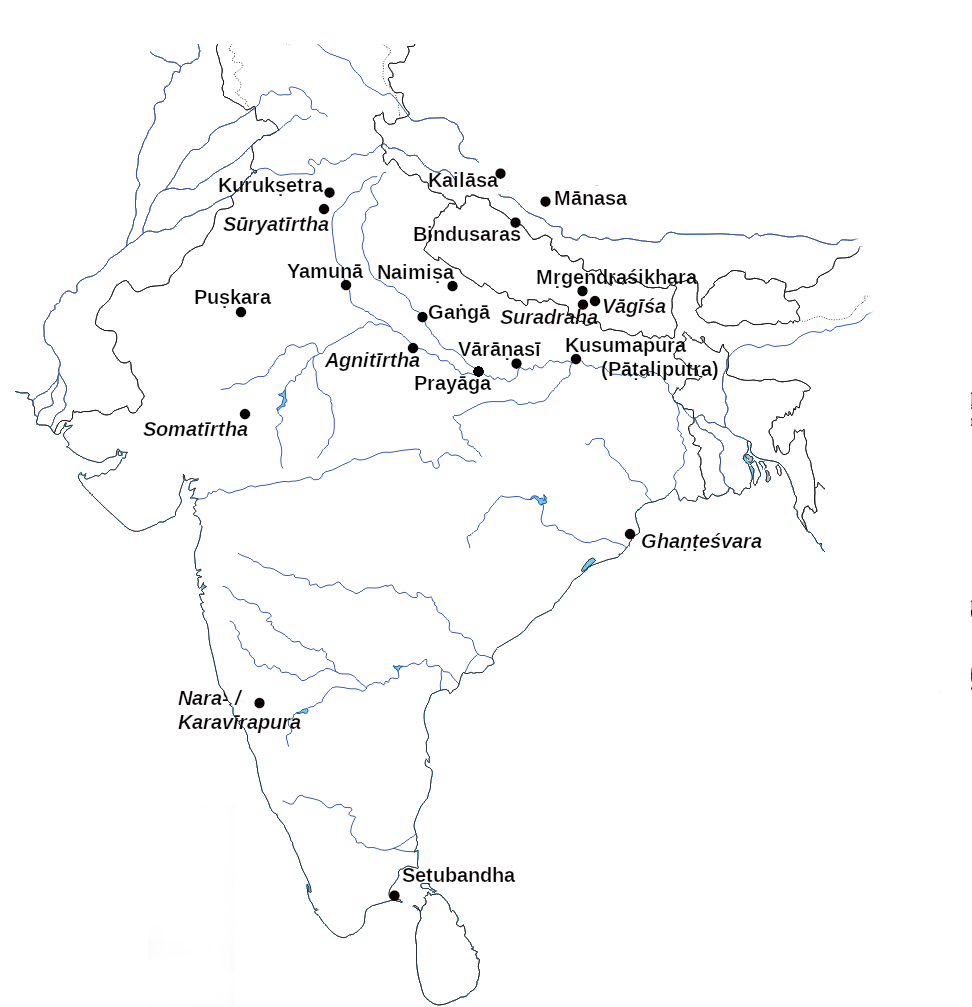
\includegraphics[scale=.35]{images/simplemap.png}
\caption[Geography of the \VSS]{A possible reconstruction of the  geography of the \VSS. Toponyms in italics are uncertain. Map constructed using a simple hydrographic map made by Daniel Dalet (d-maps.com).\label{fig:map01}}
\end{figure}

\begin{figure}[!]
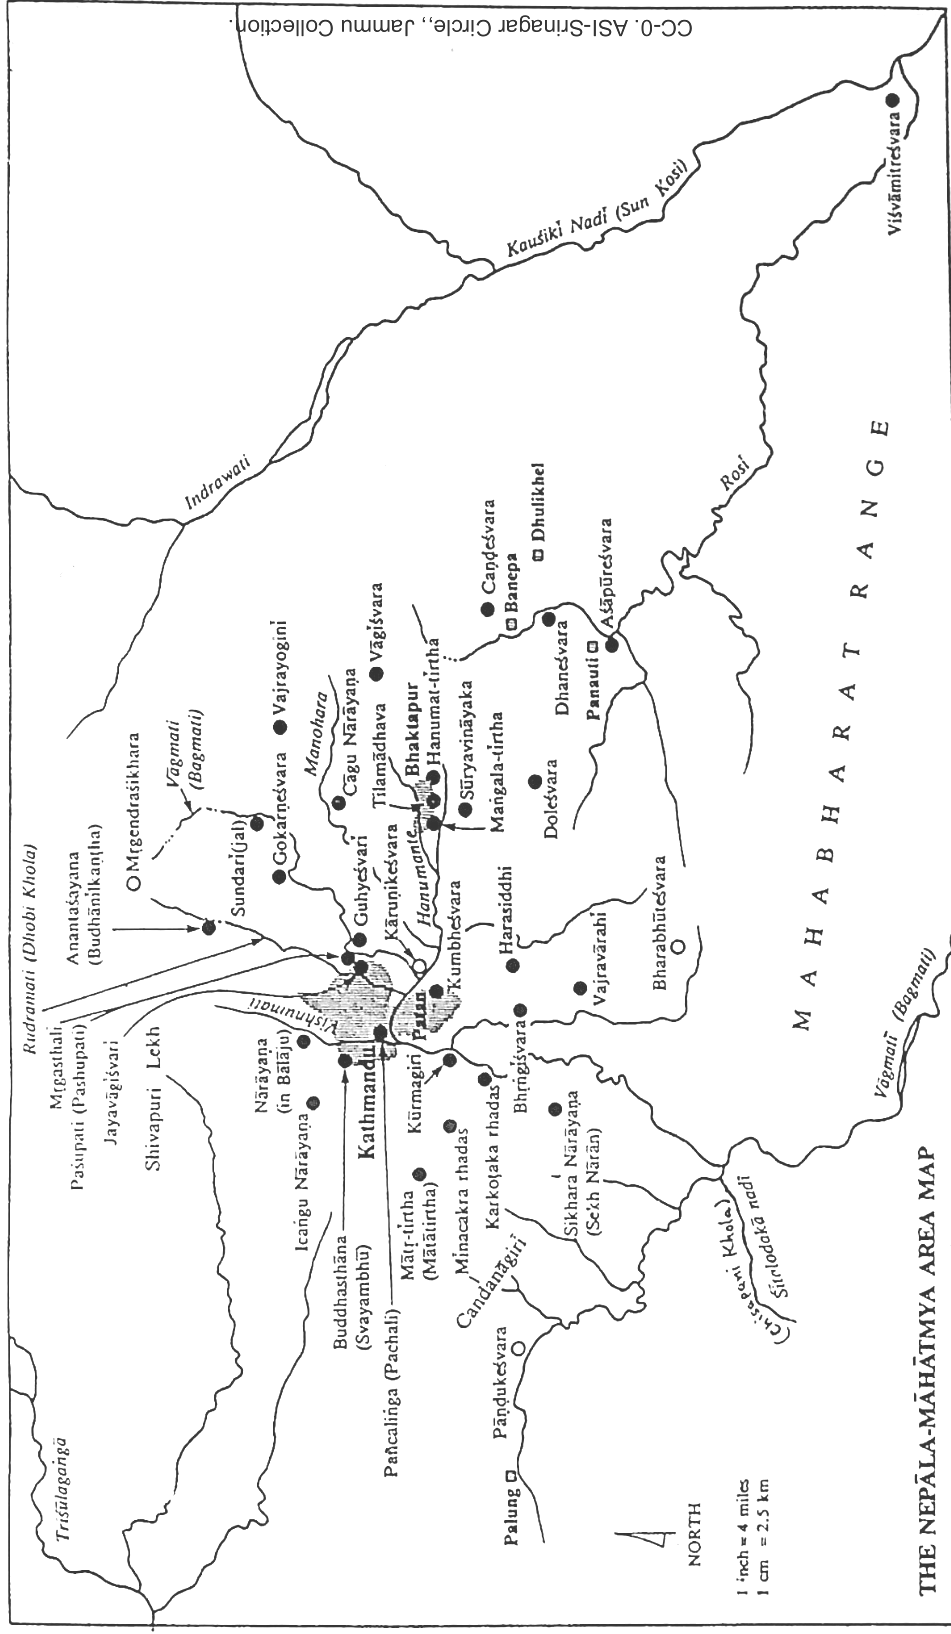
\includegraphics[scale=.40]{images/map_in_jayaraj.png}
\caption[Map in \mycite{AcharyaNepalaMahatmya}]{Map in \mycite{AcharyaNepalaMahatmya}
\label{fig:map02}}
\end{figure}


The location with which the ascetic Anarthayajña
is connected strongly suggests the Kathmandu 
valley as the geographical focus of the \VSS\
because he is a key figure and 
main interlocutor in the \VSS,
possibly the reason behind the composition of the text.%
	\footnote{On Anarthayajña's central role in the \VSS,
			see more in \mycite{KissVolume2021}.}


Turning to names of individuals mentioned in the \VSS,
those that might betray anything about the place or
time of composition of the text include King Siṃhajaṭa
and queen Kekayī, rulers of Nara- or Karavīrapura
in the narrative of chapter twelve. Unfortunately,
so far I have not been able to link these names to
any historical or legendary persons. The name of the
hero of the same chapter, Vipula,\label{Vipula} may be familiar 
from \MBH\ 13.40.16--13.43.16.: 

\begin{quote}
Devaśarman asks his disciple,
Vipula, to protect his wife, Ruci, primarily from Indra's
amorous advances, while he is away from home.
Vipula decides that the only way he can protect Ruci
is from within, i.e., by entering her body by yogic powers.
Vipula succeeds in protecting Ruci's reputation and 
departs to practise extreme austerities. Later he 
encounters several people (in fact,
as we learn later, Day and Night,
and the six seasons) who mention `Vipula's path leading to
the other world' (\skt{vipulasya pare loke yā gatis}, 
\MBH\ 13.42.27cd) as something horrible. He 
wonders what sins he may have committed that
could yield such unfortunate consequences. He
realizes that by not telling Devaśarman that he
actually entered Ruci's body, he lied and thus
may have committed a horrible sin. When Devaśarman learns
about this, he praises Vipula for his services instead, 
and all three, Devaśarman, his wife, and Vipula,
go to heaven.%
		\footnote{See a summary of Vipula's story in the 
			\MBH\ also in 
			\mycitep{SukthankarCriticalStudies}{317--318}.}
%(\MBH\ 13.43.16)
\end{quote}

\noindent
Thus, ironically, while the Vipula of the \MBH\ is famous
for protecting somebody else's wife,  
a rather different Vipula
in \VSS\ chapter twelve donates
his own wife to a Brahmin as soon as the latter expresses
interest in her. It is more than possible that
the two characters have no connection at all.%
	\footnote{Nevertheless, see the word \skt{vipule} used
	in \VSS\ 12.155b potentially referring to the famous
	story in the \MBh.}

Other characters in \VSS\ chapter twelve---Kapila, 
Vipula's father;
Bhīmabala, a traveller; Puṇḍaka, the foreman of the guild;
and Caṇḍa and Vicaṇḍa, two royal envoys---seem 
to be of little use for us to ascertain the time and place of composition or redaction of the \VSS. 

Going further, as mentioned above, any discernible influence
of a local, vernacular language on the style or grammar of
a Sanskrit work could also be useful to
locate the text in question geographically. 
The language of the \VSS\
displays numerous oddities that could be
explained by the interference of some other 
language, most likely early classical Newar.
On this, see a separate section below on 
pp.~\pageref{newar}ff.

In addition, the quotes from \Manu\ in the \VSS\
usually contain variants that can be found in the apparatus
in Olivelle's critical edition of \Manu\ (\citeyear{OlivelleManu})
as belonging overwhelmingly to
what Olivelle calls the `Northern Transmission.'%
		\footnote{See, e.g., \skt{pāpakṛt} in \VSS\ 3.34d 
		(${\approx}$\ \Manu\ 5.52) attested in Olivelle's
		Devanāgarī MSS Pu$^{5}$, Pu$^{7}$, Pu$^{9}$;
				\skt{nānyatra manur abravı̄t} in \VSS\ 3.35d 
				(${\approx}$\ \Manu\ 5.41) attested in
			Śāradā MSS {\tiny S}Ox$^{1}$, {\tiny S}Pu$^{6}$ and 
			Devanāgarī MS Tr$^{2}$;
			\skt{kūṭa} in \VSS\ 4.79 (${\approx}$ \Manu\ 11.57) in
			a MS from Kathmandu ({\tiny B}Kt$^5$), 
			in Devanāgarī/Old Nāgarī MSS
			(Lo$^{4}$, {\tiny N}Pu$^{1}$, Pu$^{2}$, Pu$^{4}$, Pu$^{10}$),
			as well as in two South-Indian MSS ({\tiny G}Md$^1$, 
			{\tiny T}Md$^3$).}
This again confirms a North-Indian or Nepalese
origin for the \VSS.

\medskip
\noindent
\label{dating}The obvious \textit{terminus ante quem} for the
composition or redaction of the \VSS\ 
is the date of the earliest MSS that transmits it.
The earliest dated MS containing the \VSS\ is \msKoa,
dated to Nepal Saṃvat 156, i.e., 1035-36 \CE.% 
	\footnote{See \mycitep{SastriCatalogue5}{721} and
		\mycitep{UmaSivaPlay}{591}. The date
	 	is clearly visible as `\skt{samvat} 156' 
	 	in the last line of the penultimate folio side 
	 	of \msKoa/8.}
In a multiple-text MS%
	\footnote{See more detail on this MS, which is
						now to be found in Munich, in	
					    \mycite{HarimotoMunichMS}.}
that is potentially earlier than \msKoa,
the \VSS\ is written in a hand that appears later than
that used for some of the other texts in that MS.%
		\footnote{\mycitep{HarimotoMunichMS}{597--598}:
		`This Śivadharma ms consists 
		of two major parts, easily distinguishable by different 		
		hands: one that appears to be produced in
		9th-c.\ Nepal [\dots], and another seemingly from 
		a century or so later [\dots] 
		The next set of folios making up this Śivadharma ms 	
		consists of three titles: the 
		\textit{Uttaromāmaheśvarasaṃvāda}* (24 folios), 
		the \textit{Vṛṣasārasaṃgraha} (50 folios), and the
		\textit{Dharmaputrikā} (11 folios). We do
		not know the original order of these three works 
		because each section starts with folio 1. Moreover, even 
		though these three titles appear to be written by the same 
		hand (probably somewhat later than the first part), there 
		is no certainty that these folios were produced to 	
		complement the first part.'}
The final colophon of the \VSS\ (and the \DHARMP) in
this MS  (\fol50r) is followed by the date
[Nepāla] `\skt{samvat} 192,' i.e., 1071-1072 \CE.

These two MSS make it impossible to date the \VSS\ later 
than the first half of the 11th century \CE, and parts of the text
may be considerably older.
Archaic features that may indicate 
that the \VSS, or parts of it, were
composed much earlier than the early 11th century
include the following. Chapter ten,%
		\footnote{Also verse 11.21.} 
while it teaches the yogic tubes
\ie{nāḍī} Suṣumnā and Iḍā, is silent on Piṅgalā, 
which is a situation similar to that in 
the 6-7-century \NisvNaya%
	\footnote{\mycitep{NisvasaGoodall}{33--35}.}  
(see details in the notes to the translation).
Similarly, 11.23a (\skt{nivṛttyādi caturvedaś}) mentions four
Śaiva \skt{kalā}s, instead of the expected and 
somewhat later, and in character tantric, five, namely
\skt{nivṛtti}, \skt{pratiṣṭhā}, \skt{vidyā}, 
\skt{śānti}, and \skt{śāntyatīta}. In the same chapter,
the order in which the \skt{āśrama}s are taught
(\skt{gṛhastha, brahmacārin, vānaprastha, parivrājaka}) 
is reminiscent of \Apastambadharmasutra\ 2.9.21.1,
and is relatively rare,
as opposed to the traditional order (\skt{brahmacārin,
gṛhastha, vānaprastha, parivrājaka}) found, e.g., in
\MANU. (See \mycitep{KissVolume2021}{195--196}.)
%cf. \mycitep{SaivaUtopia}{23}, Chapter 11, Śaiva
Another feature that might point towards a date
considerably earlier than the 11th century is the 
system of \skt{tattva}s in chapter 20:
the \skt{mahābhūta}s of classical Sāṅkhya are called 
\skt{dhātu}s here, the \skt{tanmātra}s of
classical Sāṅkhya are called \skt{guṇa}s,%
		\footnote{In contrast with, e.g.\ \SDHU\ 10.40--46 and
					\UUMS\ chapter 5, \DHARMP\ 1.42--43, or the \SIVAUP.}
the \skt{buddhi} of classical Sāṅkhya
is called \skt{mati}, and the highest \skt{tattva} 
is singular unlike the multiple \skt{puruṣa}s of classical 
Sāṅkhya. These may well be archaisms 
included in the \VSS\ consciously, but they could also
indicate that the time of composition of the \VSS\
is much closer to pre-classical Sāṅkhya than what the MS
evidence suggests.%
	\footnote{There are also numerous borrowings in \VSS\ 20
					from the Śāntiparvan of the \MBH. See more details
					at the analysis of \VSS\ chapter 20 in volume two.}

All in all, in light of all the above,
it is difficult to be more precise on the dating
of the \VSS\ than saying that its production must have
happened before the end of the 10th century, or the beginning
of the 11th century \CE\ if our oldest dated MS that transmits
the \VSS\ is close in time to the actual composition or
redaction of the text. The date could also be considerably
earlier than the 10th century, and therefore a tentative dating
for the \VSS\ would consider the 7th to 10th centuries \CE.
%    varṇas and the Liṅgapurāṇa
%    check lists of deities such as Vasus
%  bull, Nandi




% start of CGPTed section

\section{Language}\label{language}

\subsection{Newar influence?}
\label{newar}

The oddities of the language of the \VSS\ go beyond the idiosyncrasies of epic Sanskrit.
This dialect exhibits some similarities to Śaiva Aiśa Sanskrit,%
		\footnote{On Aiśa, see, e.g., \mycitep{GoodallKirana}{lxv\thinspace ff.}, 
								  \mycitep{TorzsokSYMthesis}{xxvi\thinspace ff.},
						          \mycitep{KissBraYa}{77--87}, 
						          \mycite{GerstmayrAisa}, and
						          \mycitep{HatleyBraYaVol1}{28ff.}} 
and frequently applies peculiar metrical licences, 
alongside a special vocabulary, morphology, and syntax.
Analysing this language could, ideally, help us
define the identity of the author(s) or redactor(s) of the text
and confirm our views on its place of composition.

To support a working hypothesis, I will mention parallels
between the language of the \VSS\ and early classical 
Newar---since the \VSS\ was most probably produced in the 
Kathmandu valley%
		\footnote{See pp.~\pageref{provenance}\thinspace ff.}%
---whenever possible. (This is not to suggest that the phenomena
discussed must necessarily originate in  Newar influence;
other local Prākṛts may also have played a role.)
Of course, the assumable date
of the composition of the \VSS, which is without much doubt
pre-early-11th century, does not allow any direct
comparison with contemporary Newar language texts.%
	\footnote{The earliest dated Newar document is 
			the Ukū Bāhāḥ land grant palmleaf manuscript from
			1114 \CE. See, e.g., \mycite{MallaUku}.}
Therefore I have to project a much later Newar grammar
onto an earlier and less well-known 
state of the language, which is not without risks.

In the following, I will only give a brief overview of the most
important phenomena. For details, see the observations 
on the constitution of the Sanskrit text in the footnotes 
to the translation, as well as the Index.


\subsection{Number and gender}\label{number}
One of the most evident deviation from Pāṇinian grammar in 
the text of the \VSS\ is a general disregard of grammatical concord 
in number and gender.%
	\footnote{Compare Kölver's introductory remarks in his investigation of
	`Newarized Sanskrit' (\citeyear{KolverErgative}, 202) in the \SvayP\ thus (ibid. 192):
					
					\noindent
	          	`Number is often ignored
	          	
					[\skt{catvāro 'pi maṇḍalañ ca} 429,19 (cf.\thinspace 429, 21), 
					\skt{narāḥ pañcagatiñ ca na labhec ca} 428,12],
					
					\noindent
					as is gender
					
			[\skt{tvam ekam āgataṃ na hi} 464, 10 `only you have not come’; 
			\skt{°nāgakanyā \dots\ vṛṣṭipūrṇaṃ kṛtam} 470, 8 
					`the Nāga girl made (it) full of rain'],
				
				\noindent
				and case
				
				[\skt{manuṣyāḥ \dots\ tasmai \dots\ pūjitam} 426, 2 etc. 
				`men worshipped him; he was worshipped by people'; 
				\skt{bhavatām apy arthāya karomy upāyakam mayā} 452, 5 
				`I am making an expedient for your sake'].'}
See, for example, a plural verb
(perhaps metri causa) with a singular subject in \VSS\ 1.25ab:

\begin{quote}
\skt{rātryāgame pralīyante jagat sarvaṃ carācaram} 

When [Brahmā's] night falls, the whole moving and unmoving universe dissolve[s].
\end{quote}

\noindent
Or a neuter plural participle picking up a 
neuter singular and a feminine singular noun in 1.61ab:

\begin{quote}
\skt{pramāṇaṃ nāma saṃkhyā ca kīrtitāni samāsataḥ}

The numbers [pertaining to] the measurements have been taught in brief.
\end{quote}

\noindent
Another clear example is 6.12c, where grammatical gender
is totally ignored: 

\begin{quote}
\skt{kāni lokāḥ prapadyante}

Which worlds can be attained?
\end{quote}

\noindent
Even when the \VSS\ appears to quote from the \BhG,
it tends to cause confusion for no evident reason:

\begin{quote}
        \skt{anudvegakarā vāṇī priyaṃ satyaṃ hitaṃ ca yat} (\VSS\ 6.21ab)

        \skt{anudvegakaraṃ vākyaṃ priyaṃ satyaṃ hitaṃ ca yat} (\BHG\ 17.15ab)

\end{quote}

\noindent
This line in the Bhandarkar critical edition of the \MBH\ does not 
have any significant variants, and the \VSS's version is much
more problematic grammatically than the assumable source---one can only wonder why.

This confusion---or often metrically motivated disregard---of standard Sanskrit
grammar when dealing with number and gender becomes almost
predictable when a noun phrase involves numerals.%
    \footnote{I am thankful to Judit Törzsök, who first pointed out to me
    the regular nature of the phenomenon itself as seen in the \VSS, and who 
    later drew my attention to the similar Newar grammatical rule
    (personal communication, Nov 29, 2023), which 
    led me to an investigation of a possible link between the Sanskrit of the \VSS\
    and classical Newar.}
See, e.g., verse 1.2cd:


\begin{quote}
\skt{parva cāsya śataṃ pūrṇaṃ śrutvā bhāratasaṃhitām}

Having listened to the \titleface{Mahābhārata},
to all its hundred section[s] \ie{parvan}\dots
\end{quote}

\noindent
Here, one would expect either a plural genitive \ie{parvāṇāṃ śataṃ},
a compound \ie{śataparvāṇi}, or a plural accusative \ie{parvāṇi śataṃ}.
Similarly, \skt{gatiś ca pañca vijñeyāḥ} in 3.5a stands for
\skt{gatayaś ca pañca vijñeyāḥ} (`and the paths are to be known as five'), 
partly metri causa; and an interrogative quantifier (\skt{kati}, `how many?') can
trigger the same: \skt{gatis tasya kati smṛtāḥ} (3.1d; `how many are its path[s]?').
It is worth noting that classical Newar rarely applies
any plural marker in noun phrases with numerals.\label{singularwithnumerals}% 
	\footnote{See, e.g., \mycitep{JorgensenGrammar}{18}:
			`The plural ending is wanting where plurality is expressed 
			in other ways; thus always after numerals, and
			mostly after nouns denoting ``many, all'' '.
			 Incidentally, singular after numerals is also the norm in Modern Nepali,
									 and in other, even more distant languages
									 such as Hungarian.} 
Moreover in Newar, `nouns denoting inanimate objects 
are indifferent as to number.'%
	\footnote{\mycitep{JorgensenGrammar}{5 and 17}.}
A further clear example is verse 3.6cd:

\begin{quote}
\skt{tasya patnī mahābhāgā trayodaśa sumadhyamāḥ}

       He has thirteen beautiful wives with nice waists.
\end{quote}

\noindent
Here, with no variants in any of the manuscripts consulted, only the very end 
of the noun phrase \ie{sumadhyamāḥ} bears the required 
plural ending. This again is what we often observe in Newar.%
		\footnote{`Any case [\dots] and/or plural markers [\dots], as well as 
		postpositions [\dots], are added to the last constituent of the 
		N[oun ]P[hrase].' (\mycitep{OtterCourse}{11--12}.)
		E.g.: in the Newar phrase \skt{thwo khuṃ-na khaṅ-ā rājā-pani}
		(`these kings seen by the thief'), the only indication that
		multiple kings are involved is the plural marker \skt{-pani}
		at the end (ibid.).}
A good example of total number-blindness is 5.17cd: 

\begin{quote}
\skt{kīrtitāni viśeṣeṇa śaucācāram aśeṣataḥ}

\dots\ the practice of purity is definitely expounded in great detail.
\end{quote}

\noindent
Note that there would have been little difficulty in composing the same
line in standard Sanskrit, e.g., beginning with \skt{kīrtitaṃ ca\dots}
Instead, this line betrays the author's indifference
towards grammatical concord.%
		\footnote{Compare Kölver's remark on the phrase \skt{āgataḥ sarve nāgāḥ}
		in a verse in the \SvayP\ (on p.~459 in \mycite{SastriSvayambhuP}):
		`this is a remarkable lack of sensitivity as to the category of number'
		(\mycitep{KolverErgative}{195}).}
It is also possible that the participle \skt{kīrtitāni} here
functions as a finite verb in the plural: `they teach [the practice of purity].'
In this case, there is some sense of number, but coupled with a
blurred boundary between active finite verbs and passive participles.

A special case occurs when the text appears to quote from an external source
but chooses to change the plural to the singular. E.g., \VSS\ 4.77 cites
\Manu\ 11.55, a verse that also features in the \MBH\ and in the \YAJNS.%
                \footnote{\MANU\ 11.55 (in Olivelle's edition):
                    \skt{brahmahatyā surāpānaṃ steyaṃ gurvaṅganāgamaḥ |
                         mahānti pātakāny āhuḥ saṃsargaś cāpi taiḥ saha ||};
                          \MBH\ Suppl. 12.30:
                    \skt{brahmahatyāṃ surāpānaṃ steyaṃ gurvaṅganāgamam |
                         mahānti pātakāny āhuḥ saṃyogaṃ caiva taiḥ saha ||};
                          \YAJNS\ 3.228:
                    \skt{brahmahā madyapaḥ stenas tathaiva gurutalpagaḥ |
                            ete mahāpātakino yaś ca taiḥ saha saṃvaset ||}.}
In all its versions, \skt{pāda} c of this stanza contains a plural when
labelling a list of the five `grievous sins,' except in the \VSS,
which prefers a singular.%
                \footnote{\VSS\ 4.77:
               \skt{brahmahatyā surāpānaṃ steyo gurvaṅganāgamam |
                    mahāpātakam ity āhus tatsaṃyogī ca pañcamaḥ ||}.}

There seems to be a marked tendency towards the singular in the \VSS's language. 
In general, gender confusion, and to a certain degree number confusion, are
not unusual in epic Sanskrit and in Aiśa Sanskrit,%
		\footnote{See, e.g., \mycitep{OberliesEpicSkt}{121, 292--304}, and
                \mycitep{KissBraYa}{81 and 85, and the Index therein}.}
but their extent in the \VSS\ suggests a very strong external influence---presumably
that of classical Newar.									





\subsection{Case and syntax}

An extreme example of a total disregard for Sanskrit syntax is found in \VSS~17.20:

\begin{quote}
\label{extremelanguage}
\skt{bhūmipradātā dvija hīnadīnaḥ}\\
\skt{\phantom{aaa}samṛddhasasyo jalasaṃnikṛṣṭaḥ} |\\
\skt{sa yāti lokam amarādhipasya}\\
\skt{\phantom{aaa}vimānayānena manohareṇa} ||

He who donates to a poor and distressed Brahmin land that yields plenty of corn and is in the vicinity of water will go to the world of the king of the immortal ones [i.e.\ of Indra] on a fascinating \ae rial vehicle.
\end{quote}            
            
\noindent            
Surprising as this translation may seem, it is, judging from the context, rather secure. 
\skt{Pāda}s ab probably stand for what, in more standard Sanskrit, would read:
\skt{dvijāya hīnadīnāya sasyasamṛddhāṃ jalasaṃnikṛṣṭāṃ bhūmiṃ yo dadāti}.
Instead, the phrase is constructed with what looks like a series of nominatives and a
vocative, with little or no regard for the expected case endings: endings seem to function more
as decorations than as grammatical markers.

This is difficult to explain purely in terms of Newar influence, since classical Newar does have
a dative case marker (added to the genitive for animate nouns). 
It is also striking that \skt{pāda}s cd of the same verse are composed in perfectly standard Sanskrit.%
		\footnote{See a similarly puzzling situation in the \BraYa, 
                 which is briefly described in \mycitep{KissBraYa}{74} as follows:
		`One of the most intriguing questions concerning the Bra[hma]Yā[mala] 
		is not why its language deviates from Pāṇini so often 
		but rather why sometimes it falls back to perfectly standard 
		Pāṇinian language for fairly long passages.'}

There are dozens---if not hundreds---of syntactical oddities in the \VSS,
even if not all are as baffling as the example above.%
		\footnote{Most of them are addressed in the footnotes to the translation.}
Somewhat similarly to what Kölver describes in 
his analysis of the language of the \SvayP, a Nepalese composition (\mycite{KolverErgative}),
there often (but not always) appears to be a lack of understanding of the
passive,\label{confusedpassive} 
coupled with the application of the ergative,\label{ergative} one of the
basic syntactical tools of classical Newar. 

A good example is found in 12.113cd:

\begin{quote}
\skt{indreṇāsmi phalaṃ dattaṃ sa phalaṃ datta me bhavān} 

It was Indra who gave me the fruit and I gave that fruit to you.
\end{quote}

\noindent
Again, this is the translation that seems to fit the context. 
Here the skeleton of \skt{pāda} c is a well-constructed passive:
\skt{indreṇa phalaṃ dattaṃ}, but then, instead of adding a dative or 
genitive (e.g., \skt{indreṇa me phalaṃ dattaṃ}), the author chooses 
a finite verb (\skt{asmi}). In \skt{pāda} d, after seemingly 
treating \skt{phalaṃ} as a masculine noun, and leaving
\skt{datta} in \stemform\ metri causa, and using \skt{me} for \skt{mayā},%
		\footnote{This often happens in epic Sanskrit, see 
			\mycitep{OberliesEpicSkt}{4.1.3, pp.~102--103}.}
this time he ends the phrase with a noun in the nominative \ie{bhavān} instead of
the dative or genitive. Why not write \skt{dattaṃ tad eva te mayā},%
		\footnote{Although this solution carries the metric fault of being iambic.}
or \skt{dattaṃ tava tad eva ca}?

\label{kathita}Constructions with \skt{datta}/\skt{kathita} plus an expected dative 
are especially prone to confusion. See, e.g., \VSS\ 1.62cd--63ab and 10.2d:

\begin{quote}
\skt{brahmaṇā kathitaṃ pūrṇaṃ mātariśvā yathātatham}\\
\skt{vāyunā pāda saṃkṣipya prāptaṃ cośanasaṃ purā}

        [The Purāṇas] were taught by Brahmā to 
        Mātariśvan [= Vāyu] in their entirety, in their true form.
        Vāyu abridged the verses and then gave [them] to Uśanas.
        
\skt{bravīmi vaḥ purāvṛttaṃ nandinā kathito 'smy aham}

        I shall teach you an ancient legend that Nandi told me.
\end{quote}

\noindent
Again, there is some struggle first with an expected dative here:
it ends up in the nominative \ie{mātariśvā}. Then an expected 
agent in the instrumental, or rather another dative, 
becomes an accusative \ie{uśanasaṃ}. Thirdly,
\skt{kathito 'smi} stands for \skt{kathitaṃ mama} or
\skt{kathitaṃ mahyam}. 

Somewhat similar are constructions with a 
past participle plus \skt{asmi}
in place of an active finite verb. See, e.g.,
13.68cd, 14.56ab and 15.15cd:

\begin{quote}
\skt{eṣa garbhasamutpattiḥ kathito 'smi varānane}

            This is how I have told you the formation of 
            the embryo, O Varānanā.
            
\skt{āgneyadhātuṃ somaṃ ca kathito 'smi varānane}

			I have taught, O Varānanā, the Fiery constituents 
			and the Soma-ones.
			
\skt{kathito 'smi samāsena kim anyac chrotum icchasi}

		Thus have I briefly described [to you, O Mahādevī, the soul.] 
		What else would you like to hear?
\end{quote}

\noindent
These resemble a phenomenon \citeauthor{JorgensenVicitra}
observed in a Sanskrit passage in the Newar
\VicitraKAU, where the phrase \skt{na jñāto 'ham}\label{najnatoham} must be interpreted
as `I did not know.'%
		\footnote{\mycitep{JorgensenVicitra}{77 and 328}.\label{najnatohamfn}
						Compare \skt{tat phalaṃ sa niveditaḥ} (`he gave that fruit') in \VSS\ 12:67d.}

%Vicitrakar :
%ibid and 66 \skt{aṣṭhan/au divasam āgata} should mean `Come on the eighth day'.;
%buddhamārgaṃ abhijñātaṃ: `on the well-known path of the Buddhas'
%80 and 328-329 samagraṃ, stem forms etc.!?

Occasionally, the agent of an active construction with a transitive verb
simply imitates an ergative structure: \skt{viṣṇunā\dots\ papraccha} (1.8),
\skt{dhanyās te yair idaṃ vetti} (4.75ab),
\skt{sa}[!] \skt{hovāca pathīkena} (12.60a).%
		\footnote{This happens also in Aiśa. See, e.g., \SiddhYogMata\ 18.23: 
		\skt{pūjayet \dots\ mantriṇā} (\mycitep{TorzsokSYMthesis}{42}).}
%yajec cakre ca vidhivad yoginīsiddhim icchatā 21.12cd

\label{tellplusgen}Another typical syntactical pattern in the \VSS\ is a verb
meaning `to tell, teach' followed by a noun in the genitive. See, for example, 4.69ab:

\begin{quote}
\skt{caturmaunasya vakṣyāmi śṛṇuṣvāvahito bhava}

        I shall tell you about the four cases of observing silence. 
        Listen, be attentive.
\end{quote}

\noindent
One could argue that \skt{pāda} a is simply elliptical and that
a verb like \skt{lakṣaṇaṃ} or \skt{svabhāvaṃ} 
(`the characteristics/\thinspace essence [of X]') is missing. 1.37ab and 4.17ab
display similar structures:

\begin{quote}

\skt{brahmāṇḍānāṃ prasaṃkhyātuṃ mayā śakyaṃ kathaṃ dvija}

How could I enumerate [all the details of] the Brahmāṇḍa[s], O twice-born?

\skt{evaṃ satyavidhānasya kīrtitaṃ tava suvrata}

Thus have [I] taught you the rules of truth, O virtuous one.

\end{quote}

\noindent
This phenomenon is difficult to explain as the result of Newar influence, since
classical Newar would usually also require an extra word (such as \skt{khaṃ} `thing, topic, word, story') 
in such constructions. While it may fall into one of the categories that 
Jørgensen (\citeyear{JorgensenGrammar}) describes in his \S 26 g, h, and i, 
where he gives examples of the use of the genitive,
it is more plausibly part of a broader class of phenomena that Edgerton,
in his discussion of Buddhist Hybrid Sanskrit,
labels `genitive with miscellaneous verbs.'%
		\footnote{\mycitep{EdgertonHybrid}{vol.~1, \S 7.65, p.~47}.}


These kinds of deviations from standard Sanskrit syntax require that 
the translation be, to some extent, intuitive and context-driven,
rather than mechanically adhering to the rules of standard Sanskrit grammar.%
        \footnote{Kölver's `dative for direct object'
                (\mycitep{KolverErgative}{195, 4.2.1(b)}), i.e. constructions such as 
                \skt{tasmai prapūjitam} meaning  'X worshipped him,' cannot be found in the \VSS.
                Although the \VSS\ is obviously earlier than anything Jørgensen describes,
                it may be of some interest that according to him (\citeyear{JorgensenGrammar}, \S 27b),
                this is a late phenomenon in Classical Newar.}

%end of CGPTed section

\subsection{Cardinal and ordinal numbers}

Although the \VSS\ does use simple ordinal numbers such 
as \skt{prathama}, \skt{dvi\-tī\-ya}, and \skt{tṛtīya}, with higher 
numbers there seems to be no clear distinction between cardinal and ordinal usage:
cardinals are frequently used where ordinals would be expected.
See, for example, 20.8ab and 11ab:

\begin{quote}
\skt{caturviṃśati yat{ }tattvaṃ prakṛtiṃ viddhi niścayam}\\
\skt{dvāviṃśati ahaṃkāras{ }tattvam{ }uktaṃ manīṣibhiḥ}

Know the twenty-fourth Tattva certainly as Prakṛti.
The twenty-second Tattva is Ahaṃkāra according to the wise.
\end{quote}

\noindent
This phenomenon is known, to some extent, from epic Sanskrit,%
	\footnote{See \mycitep{OberliesEpicSkt}{\S 5.2.2, pp.~127--128}.}
but is even more characteristic of classical Newar.%
		\footnote{See \mycitep{JorgensenGrammar}{42} and \mycitep{OtterCourse}{57}.}



\subsection{Stem form nouns}\label{stemform}

\Stemform\ nouns, or uninflected nominal bases (\skt{prātipadika}s), are extremely common in the
language of the \VSS. While such forms are not alien to the Aiśa Sanskrit of Śaiva Tantras,%
		\footnote{See, e.g., \mycitep{KissBraYa}{75--77} and \mycitep{NisvasaGoodall}{126 and 441}.}
the sheer frequently in the \VSS\ is striking and reminiscent one of the zero suffix of the nominative and accusative---or
rather of the `casus indefinitus' or `absolutive case'---of classical Newar.%
		\footnote{\mycitep{JorgensenGrammar}{18 and 21}, and \mycitep{OtterCourse}{16}.} 
Very often, these uninflected forms are required to restore the metre, making them difficult to emend.
Moreover, they frequently they blend in \skt{sandhi} with the following word, thus reinforcing their presence.

See some clear-cut examples, with the expected but usually unmetrical standard form in parentheses, include:

\begin{quote}
1.63a: \skt{vāyunā pāda saṃkṣipya} (\skt{pādaṃ}) \\
1.63c: \skt{tenāpi pāda saṃkṣipya} (\skt{pādaṃ}) \\
2.25c: \skt{bhogam akṣaya tatraiva} (\skt{akṣayaṃ}) \\
2.26d: \skt{īśānānāṃ smṛtālayaḥ} (\skt{smṛta ālayaḥ}) \\
4.19f: \skt{prasahyasteya pañcamam} (°\skt{steyaṃ}) \\
4.72a: \skt{caturdhyānādhunā} (°\skt{dhyānam adhunā}) \\
4.77a: \skt{pramādasthāna pañcaiva} (°\skt{sthānaṃ} or °\skt{sthānāni})
 \\
6.5c: \skt{vedādhyayana kartavyaṃ} (\skt{vedādhyayanaṃ}) \\
6.14a: \skt{dvitīyaṃ tattva puruṣaṃ} (\skt{tattvaṃ}) \\
\end{quote}




\subsection{Vocabulary}

The special vocabulary of the \VSS\ includes the following:
\skt{karhacit} for \skt{karhicit} (in some MSS in 4.3b, and 4.47b): 
        see \mycitep{EdgertonHybrid}{vol.~2, s.v. \skt{karhacid}}; 
\skt{hṛdi} as nominative 10.27cd, 20.17a, 22.24ab: 
        see \skt{diśi} in Aiśa, \mycitep{KissBraYa}{83};
\skt{tirya} for \skt{tiryañc/tiryak} (3.5c, 4.6a, 4.30a, 8.4c, 12.150,\linebreak
 18.12, 18.15, etc.);
\skt{me} instead of \skt{mayā} (8.30d, 11.4b, 12.24b, 12.55a,\linebreak
 12.113d, etc.): 
        see \mycitep{OberliesEpicSkt}{4.1.3 [pp. 102--103]};
\skt{āhūta}[\skt{saṃ}]\skt{plavana} for \skt{ā\-bhūta}[\skt{saṃ}]\skt{plavana} (2.13a, 12.151b);
\skt{puna} for \skt{punar} (1.3a): see Middle Indic \skt{puna} mentioned in
        \mycitep{EdgertonHybrid}{vol.~2, s.v. \skt{punā}}; 
\skt{nirdeha} for \skt{videha} (1.12d);
\skt{koṭya} for \skt{koṭi} (thematisation, 1.52c);
\skt{ālayana} for \skt{ālaya} (possibly 2.3a);
\skt{īrṣyatā} for \skt{īrṣyā} (2.6d);
\skt{vaṇi} for \skt{vaṇij} (thematisation, 9.16a);
\skt{sara} for \skt{saras} (thematisation, 10.27a);
\skt{sakhāyā} for \skt{sahāyā} (12.36c);
\skt{śreṣṭhi} for \skt{śreṣṭhin} (thematisation, 12.63a, 12.80a);
\skt{śaśi} for \skt{śaśin} (thematisation, 12.110d).





\subsection{Metre}\label{metre}
\label{muta}
Perhaps the most striking metrical feature of the text is its generous use of the poetic licence sometimes labelled
`muta cum liquida,'%
	\footnote{I.e. `stop with liquid.' The term `muta' stands for a `plosive' sound or `stop'. 
	 For a recent contribution on this phenomenon, see,
 	 \mycite{SenMutaCum} (discussing it as it appears in Latin).}
 	%and \mycitep{BaloghYati}??  2018, note 6 (discussing 
 	%Sanskrit metre), Balogh 2019, 39 and 115
that is, allowing a syllable to remain light \ie{laghu} 
before certain consonant clusters that would normally render it heavy \ie{guru}.%
		\footnote{On its appearance in Śaiva Tantras,
							see, e.g., \mycitep{GoodallParakhya}{lxxxi} and
							\mycitep{NisvasaGoodall}{441}. The latter concerns
							 the syllable \skt{spa} in \skt{sparśan} in \NisvNaya\ 2.55cd:
							\skt{sparśatanmātra sparśan tu gṛhṇate tvacam āśṛtaḥ}. }
Syllables beginning with \skt{pr, br, kr}, and also \skt{hr},
especially (in theory exclusively) at the beginning of words, are well-known
candidates for this licence.%
			\footnote{See, e.g., \mycitep{ApteDict}{Appendix~A p.~1}.
			Note that even here, the phenomenon extends beyond plosive sounds:
                                \skt{h} is rather a fricative.}
In the \VSS, \skt{tr, dr, bhr, vr, śr}, and also \skt{śy},%
	\footnote{See, e.g., the cadence of 5.15b: \skt{śukaśyenakān} for \ \shortsyllable\
								\shortsyllable\ - \shortsyllable\ -}
\skt{śv, sv}, and \skt{dv}, can also trigger this phenomenon.%
                        \footnote{See \mycitep{OberliesEpicSkt}{xxxvii} for an even wider
                                range of conjuncts triggering the same in the \MBH.}
All these syllables involve conjunct consonants with
a semivowel in second position. Since the sound in 
first position is not always a plosive (`muta'), the term
`muta cum liquida' is actually less than perfect in our case.
I therefore propose the terms `\krama\ licence' or '\skt{kramasaṃyoga}.' 
To give reasons for this,
% and possibly also rpa,CHECK! seem additional ones.
% Deshpande Priestly Sanskrit 421
and for context, it is perhaps not useless to briefly show
what a well-known author on prosody, 
Kedāra\-bhaṭṭa (11th or 12th century),%
		\footnote{\mycitep{OllettGana}{333}.}
who is frequently quoted by Mallinātha, has to say on this
phenomenon in his
\skttitle{Vṛttaratnākara}{Vrttaratnakara} (here given together with Sulhaṇa's
\skttitle{Sukavihṛdayanandinī}{Sukavihrdayanandini} commentary):%
		\footnote{\mycite{PatelVrttaratnakara}.}

\begin{quote}
\skt{padādāv}%
                \footnote{Some editions read \skt{pādā}°.}
\skt{iha varṇasya saṃyogaḥ kramasaṃjñikaḥ} | \\
\skt{puraḥsthitena tena syāl laghutā 'pi kvacid guroḥ} || 1.10 ||

In this [field, i.e.\ in \skt{chandaḥ\-śāstra}], conjunct consonants
\ie{saṃ\-yoga} in a word-initial syllable \ie{padādau varṇasya} is
called a `sequence' conjunct (\skt{kra\-ma}[\skt{saṃyoga}]). 
[A syllable that counts as] heavy because one
such [consonant cluster] stands in front [of it, i.e.\ after it] can 
sometimes be treated as light.

{\footnotesize [Comm.:] 
\skt{vibhaktyantaṃ padaṃ tasya padasyādau vartamāno yo varṇas tasya
saṃ\-yogaḥ} |
\skt{sa iha śāstre kramasaṃjño jñeyaḥ} |
\skt{tena krameṇa purovartinā prākpadānte vartamānasya
prāptagurubhāvasyāpi laghutā syāt} | 
\skt{kvacil lakṣ}[\skt{y}]\skt{ānu\-ro\-dhe\-na} | 
\skt{nanu ka eṣaḥ kramo nāma saṃyoga ucyate} | 
\skt{pūrvācāryāṇāṃ piṅgalanāgaprabhṛtīnāṃ kāli\-dāsādīnāṃ ca
kavīnāṃ samayaḥ parigṛhītaḥ} |
\skt{saṃyogaḥ kramasaṃyogaḥ}
||~10~||
\skt{tatra gra-saṃyogena yathā} | 
\skt{idam asyodā\-hara\-ṇam}~|

A `word' is [a unit of speach that] ends in an inflection. 
A `conjunct' is in a `syllable' which is
at the beginning of such a word. 
`In this' field of science, it is to be known under the 
term `sequence' \ie{\krama}. By that sequence which stands in front, 
[a syllable] at the end of the previous word, even if it acquired
heaviness [by position], may acquire lightness. `Sometimes' [means:]
as required.
If you have doubts about this combination of consonants called `sequence' (\krama),
[I reply:] the old teachers such as Pi\-ṅgalanāga and poets such as Kālidāsa
accepted [this] rule. The conjunct \ie{saṃyoga}
is the sequence[-type] \ie{\krama} [i.e. word-initial]
conjunct \ie{saṃyoga} [in this case].
Among [the possibilities,] for example with the conjunct \skt{gr}.
Here is an example of that:}

\skt{taruṇaṃ sarṣapaśākaṃ navaudanaṃ picchalāni ca dadhīni} |\\
\skt{alpavyayena sundari grāmyajano miṣṭam aśnāti} || 1.11 ||

Tender mustard seed, fresh porridge, and creamy curds: men in the village eat
these kinds of savoury dishes, O pretty girl, because they do not have
much money.%
	\footnote{I.e.: `you are pretty, don't waste your time with poor village men.'}
\end{quote}

\noindent
The example verse given above (1.11) is in \skt{āryā}, and the
metric pattern of the second half-verse is, strictly speaking, the following:
 
- - | \shortsyllable\ - \shortsyllable\ | - \shortsyllable\ -!~| 
- \shortsyllable\ \shortsyllable\ | 
- - | \shortsyllable\ | -  - | - |

\noindent
For any \skt{āryā}, this is unmetrical for it yields 28 mor\ae, instead
of the expected 27. By treating the final syllable of \skt{sundari} short, 
in spite of the following \skt{grā}, the pattern conforms 
to the expected pattern: 

- - | \shortsyllable\ - \shortsyllable\ | 
- \shortsyllable\ \shortsyllable\ | - \shortsyllable\ \shortsyllable\ | - - | 
\shortsyllable\ | - - | - |

\noindent
The commentator gives several more examples, involving the syllables
\skt{gra}, \skt{hra}, and \skt{bhra}, and confirms that the rule
applies only to word-initial consonant clusters: 

\begin{quote}
{\footnotesize\skt{padādāv iti kim | anyatra mā bhūt |}

Why `at the beginning of a word'? [Because] elsewhere it should not be.}
\end{quote}

\noindent
Here follow some examples from the \VSS. The syllables 
with the \krama\ conjunct consonant, before which the syllable
is not turned into heavy, are encircled, and the metre is given in 
parentheses.

\begin{quote}	
1.1c: \skt{harīndra\Circled{bra}hmādibhir āsamagraṃ} (\skt{upajāti})\\
4.67c: \skt{prajñābodha\Circled{śru}tiṃ smṛtiṃ ca labhate mānaṃ ca nityaṃ labhed} (\skt{śārdūlavikrīḍita})\\
4.89a: \skt{iti yama\Circled{pra}vibhāgaḥ kīrtito 'yaṃ dvijendra} (\skt{mālinī})\\
5.5cd: \skt{parastrīpara\Circled{dra}vyeṣu śaucaṃ kāyikam ucyate} (\skt{pathyā})\\
5.9cd: \skt{vānaprasthasya \Circled{tri}guṇaṃ yatīnāṃ tu caturguṇam}  (\skt{na-vi\-pulā})\\
5.15ab: \skt{haṃsasārasacakrāhvakukkuṭān śuka\Circled{śye}nakān} (\skt{pathyā})\\
6.13ab: \skt{brahmalokaṃ tu \Circled{pra}thamaṃ tattvaprakṛticintayā} (\skt{na-vi\-pulā})\\
8.33a: \skt{tasmān mauna\Circled{vra}taṃ sadaiva sudṛḍhaṃ kurvīta yo niścitaṃ} 
 (\skt{śārdūla\-vikrīḍita})\\
10.31b: \skt{īśānenābhijuṣṭaṃ hṛdi \Circled{hra}da vimalaṃ nādaśītāmbu\-pū\-rṇam} (\skt{srag\-dharā})\\
11.9ab: \skt{manaḥśuddhis tu \Circled{pra}thamaṃ dravyaśuddhir{ }ataḥ param} (\skt{na-vipulā})
\end{quote}

\noindent
These indeed follow the rule of having the special conjunct with the semi\-vowel
at the beginning of a word in the sense that the word can be a member
of a compound.%
		\footnote{There are some problematic verses that I ignore here. They are
						unlikely to change the overall picture.}
As noted above, since conjuncts such as \skt{śr} and \skt{hr} show up
in this phenomenon, the phrase `muta cum liquida' is slightly misleading,
and therefore I use the phrase `\krama\ licence' instead.
To understand how unique the \VSS's indulgence in this
\krama\ licence is, the epics and the Purāṇas should perhaps 
be examined from this perspective.						

\label{short2long}Another metrical oddity, or rather, metrical licence, applied
regularly in the \VSS, exclusively in non-\skt{anuṣṭubh} verses,
 is that a word-final light syllable can count 
as heavy. Here are some examples, with the light syllable now
turned heavy encircled:

\begin{quote} 

3:42d: \skt{etatpuṇyapha\Circled{la}m ahiṃsakajanaḥ prāpnoti niḥsaṃśayaḥ} 
 (\skt{śā\-rdū\-la\-vikrī\-ḍita})\\ 
 4.5a: \skt{na narmayu\Circled{kta}m anṛtaṃ hinasti} (\skt{upajāti})%
 		\footnote{Versions of this line in the \MBH\ and the \MATSP\
 								read °\skt{yuktaṃ vacanaṃ}, avoiding the metrical
								problem (see the apparatus
 								at verse 4.5 in my edition below).}\\
4.39c: \skt{aśeṣaya\Circled{jña}tapadānapuṇyaṃ}  (\skt{upajāti})\\
4.59c: \skt{vijñānadha\Circled{rma}kulakīrtināśa} (\skt{upajāti})\\
4.59d: \skt{bhavanti vi\Circled{pra} damayā vihīnāḥ} (\skt{upajāti})\\
5.20a: \skt{śaucāśaucavidhijña mānava ya\Circled{di} kālakṣaye niścayaḥ} (\skt{śā\-rdū\-la\-vikrī\-ḍita})\\
6.18b: \skt{jijñāsyantāṃ dvijen\Circled{dra} bhavadahanakaraḥ prārthanā-\linebreak ka\-lpa\-vṛkṣaḥ} (\skt{sragdharā})\\
7.13b: \skt{saubhā\Circled{gya}m atulaṃ labheta sa naro rūpaṃ tathā śobhanam} (\skt{śā\-rdū\-la\-vikrīḍita})\\
8.44d: \skt{na bhavati punaja\Circled{nma} kalpakoṭyāyute 'pi} (\skt{mālinī})\\
11.42b: \skt{saṃsāroddhara\Circled{ṇa}m anityahara\Circled{ṇa}m ajñānanirmūlanam} (\skt{śā\-rdū\-la\-vikrīḍita})\\
11.42c: \skt{prajñāvṛddhika\Circled{ra}m amoghakaraṇaṃ kleśārṇavottāraṇaṃ} (\skt{śā\-rdū\-la\-vikrīḍita})\\
11.42d: \skt{janmavyādhiha\Circled{ra}m akarmadahanaṃ sevet sa dharmo-\linebreak ttamam} (\skt{śā\-rdū\-la\-vikrīḍita})\\
12.150c: \skt{nityaṃ rogādhivā\Circled{sa}m aniyatavapuṣaṃ trāhi māṃ kāla\-pāśāt} (\skt{srag\-dharā})
\end{quote} 

\noindent
When the syllable that is turned into heavy is followed by \skt{-m}
(see 3.42d, 4.5a, 7.13b, 11.42bcd, and 12.150c among the examples above), 
the phenomenon can be treated as the one described in 
\mycitep{EdgertonHybrid}{vol.~1, \S 2.68--69, p.~19--20}:

\begin{quote}
2.68. As in M Indic generally, anusvāra is often used
instead of any final nasal. This seems to be more than a
merely orthographic matter. For it occurs before vowels,
in what must have been close juncture [\dots] 

2.69. Most texts make use of this practice in verses
for metrical convenience. It is absolutely standard practice
in all verses to use final \skt{m} before a following initial vowel
if meter requires a short final syllable, but \skt{ṃ} if a long is
required. No editor has seen this clearly; all editions are
confused and inconsistent in this respect. So are the mss.\ to 
some extent; but they follow the rule in an overwhelming
majority of instances, and there can be no question of its
original validity; the exceptions are mere corruptions of
tradition.
\end{quote}
  
\noindent
Upon re-examination, none of the witnesses of the \VSS\ that were collated, 
or only consulted for this purpose (\msCa\msCb\msCc\allowbreak\msNa\msNb\msNc\msM\msParis\msKoa\msKob),
seems to use an \skt{anusvāra} in the above cases. There is only one exception:
\msM\ writes \skt{anityaharaṇaṃ}, °\skt{vṛddhkaraṃ} 
and °\skt{vyādhiharaṃ} in 11.42 before vowels (but not
\skt{saṃsāroddharaṇaṃ}!). The same MS has neither 
\skt{ṃ} or \skt{m} in 12.150c (°\skt{vāsa aniyata}°).
One could argue that this lack of awareness of \skt{ṃ} before
a vowel indicating \skt{gurutva} in almost all cases in all MSS
are `mere corruptions of tradition,' and then typesetting
such -\skt{m} + vowel combinations as \skt{-ṃ} + vowel 
would be commendable.
On the other hand there is little evidence that in the transmission
of the \VSS\ \skt{anusvāra}s were used in this way. This is why
I hesitate to apply `Edgerton's rule' in this edition. Another argument
against applying it is all the cases in which the syllable turned into heavy
ends in a vowel (4.39c, 4.59cd, 5.20a, 6.18b, and 8.44d among the
examples above). There can be no orthographical indication of \skt{gurutva} there;
there may have not been any need of it in the other cases either.
In general, all the metrical laxity discussed above may originate from
the authors' or redactors' insensitivity to the difference between light/short and heavy/long
syllables, or short and long vowels, possibly from the underlying Newar language. 


Against Newar: no loan words no phonetic changes like l-r
%\CHECK  a more or less full collation is important: we cannot automatically reject `ungrammatical' or unmetrical forms because they may well be  the `original' one

\CHECK the more original a section the more extreme language? see ch11



\section{Authors, redactors and target audience}

It is more than likely that the \VSS\ was produced by a group 
of authors and redactors, rather than by a single individual. 
First, the extent of the text and the variety of its topics
cast doubt on whether one author could have undertaken the task.
More importantly, the language varies from chapter to chapter:
the peculiarities of the Sanskrit used in the \VSS, as described above,
do not appear to the same degree in every the chapter. 
For example, the language of chapter three display strong signs
of a possible Newar influence, and
chapter seventeen is rather problematic and non-standard,
containing some of the most ungrammatical sentences in the entire work,%
               \footnote{See p.~\pageref{extremelanguage}.}
whereas, i.e., chapter seven is relatively well-written, in a simple and 
clear style---though still far from perfect Sanskrit.

        Thus, one could picture a group of Paṇḍits---in our case, probably in 
9-10th-century Kathmandu---none of whom possessed a high degree of mastery
in Sanskrit, likely with a Newar background, and a broad knowledge
of the \MBh, the Purāṇas, Dharmaśāstra, and some limited acquaintance
with Śaiva Tantra and Buddhism.
        They might have distributed among themselves the task of writing different 
parts of the text on various topics, in an effort to create 
a new Dharmaśāstric work that introduced some radical innovations concerning the
\skt{āśrama}-system, the \skt{varṇa}s, on Śiva's world (the Śivāṇḍa), and so forth.
Surely, the different layers of the text---general Dharmaśāstric, Vaiṣṇava,
and Śaiva---were composed by authors or redactors with varying
religious and intellectual backgrounds. 
        While each individual chapter exhibits its own linguistic and compositional issues,
the final redaction---that is, the overall design of the final structure and
the assembly of the text as we now have it---is a brilliant achievement:
transitions between chapters and between doctrinal layers
are, in most cases, not only smooth but may also
encode a hidden message, suggesting a progression from the 
everyday (Dharmaśāstra) to the religious (Vaiṣṇava), 
and from the exoteric to the esoteric (Śaiva).%
        \footnote{This is not to say that there are no evident
                  contradictions and overlaps when similar teachings in different
                  chapters are compared. For instance, one teaching
                  on observing silence \ie{mauna} gives four categories
                  (4.69), while another, similar one, gives five (8.25--33).}

As for the target audience, it is difficult to say anything definite.
One of the aims of the article \mycite{KissVolume2021} was
to search for clues regarding the r\^ole of the \VSS\ in the Śivadharma corpus;
it also touches upon the possible social milieu and intended audience(s) of the \VSS.
The conclusion  therein (pp.~200--201), focusing on the fusion of 
Vaiṣṇava and Śaiva material in the \VSS, and on the reinterpretations of 
the \skt{āśrama} system in its eleventh chapter, includes the following:

\begin{quote}
The \Vss's role in the Śivadharma corpus is then twofold: 
it provides a text that is suitable for Vaiṣṇavas and Śaivas,
presenting its teachings on different levels of an esoteric scale, 
the Śaiva teachings being closest to the core, and always
providing an internalised, secret version of topics 
discussed in the other layers; and it also reinvents the traditional 
\skt{āśrama} system in a Śaiva way,
but in such a manner that would be acceptable for other religious groups. 
This may be an attempt to further develop an idea that appears in both 
the \SDhS\ and the \SDhU.%
        \footnote{[Footnote in the original:]
        These texts use new phrases for the four \skt{āśrama}s: \SDhS\
        chapter eleven uses the terms \skt{śivagṛhāśramin}, \skt{śivabrahmacārin}, 
        \skt{śivavaikhānasa} and \skt{śivavratīndra},
        while the \SDhU\ 12.203--207 uses \skt{śivabrahmacārin}, \skt{śivāśramadharmasthaḥ}
        \skt{gṛhasthaḥ}, \skt{śivāśramavanastha}, and for the fourth category both the terms \skt{pāśupata} and
        \skt{mahāvratadhara}. On this topic, see \mycitep{DeSiminiGods2016}{52--53} and 
        Bisschop, Lubin and Kafle 2021, 17 ff. [i.e., \mycitep{SaivaUtopia}{17 ff.}]}
\end{quote}

\noindent
Indeed, one of the most striking features of the \VSS\
is its structure, in which Vaiṣṇava material frames
Śaiva teachings (see pp.~\pageref{structure}\thinspace ff. above). 
Its intended audience must have included adherents of both religious traditions.
Even the title is not unambiguously Śaiva, as previously discussed
(see pp.~\pageref{title}ff. above).
Thus, we probably cannot maintain that the text is primarily Śaiva
or that its main target was lay Śaivas.
Rather, it seeks a balance between Vaiṣṇava and Śaiva teachings, 
and this duality most likely reflects the religio\-political reality of its time.

What must be stressed is the text's radicalism in certain chapters---for example, in chapters 2, 11, and 19.
These chapters appear to deconstruct the religious duties of the householder, 
internalise the social disciplines \ie{āśrama}, and reinvent 
the origin of the social classes \ie{varṇa}, respectively.
This radicalism and innovativeness may have been among the reasons for the composition of the \VSS.

A mixture of radical innovations, an idealistic rejection of the traditional \skt{varṇāśrama}-system, and the 
praise of yogic practices and the Pāśupata tradition may have been intended to
appeal both to the lay Śaiva and Vaiṣṇava householder and to aspiring yogins and ascetics.





\section{Why was the \VSS\ included in the Śivadharma corpus?}

It is difficult to ascertain why, when and how, the \VSS\ was included in the \Sivadharmacorpus.
The corpus itself, as De Simini  (\citeyear{DeSiminiMSSFromNepal2016}, 233) writes,
`as we know it seems to be an invention of Nepal'.
To summarise the relevant part of \mycite{HarimotoMunichMS} on the formation 
of the \Sivadharmacorpus, it appears that the
earliest unit formed as a collection of texts may have comprised the \SDhS\ and
the \SDhU---two texts probably composed, or at least known, outside Nepal---and the
\SDhSangr, whose provenance remains obscure.
These were later joined by the \UMS, and then by the beginning of the tenth century \CE, 
by the \SivaUp.
This development is inferred from some of the colophons in the Munich MS (MS \msM):
the colophon of the \UMS, the fourth text in that MS---likely copied from an earlier exemplar---suggests
that the corpus was considered fourfold, whereas the colophon of the \SivaUp,
the fifth text, presents it as fivefold (\mycitep{HarimotoMunichMS}{600--603}).
In MS \msM, the \VSS\ appears to have been written in a later hand, perhaps
indicating that it was added subsequently.


The \VSS\ may have already been existence, most probably in the Kathmandu valley,
well before the beginning of the tenth century (see p.~\pageref{provenance}ff).
It was probably added to the collection after the original set of three or four
texts had been augmented with additional texts in Nepal. The \VSS\ must have been considered
a valuable work, and its survival was secured by its attachment to a 
prestigious corpus. Alternatively, it may have been commissioned by a king in Kathmandu
after a preliminary version of the corpus had already become well-known, 
in response to a perceived need to add a locally composed text.





%%% CG start %%%
\section{Contents of chapters 1--12}\label{contentsof1_12}

The following are brief descriptions of the topics covered in chapters 
1--12 of the \VSS, which have been edited and translated in this volume. 
These are accompanied by brief discussions and some analytical remarks.%	
		\footnote{See more details in the footnotes to the translation.
                          See a Sanskrit summary of the contents of the \VSS, based on Naraharinath's edition,
                          in \mycitep{AnilkumarBook}{61--72}. }

					
\subsection*{Adhyāya 1}\label{contents_of_ch01}
After a \skt{maṅgala}-verse that addresses a 
deity whose identity is obscure\linebreak
(verse 1.1; is it Śiva or the 
impersonal Brahman?), we enter the first layer 
of the text, which consists of a dialogue between Janamejaya and 
Vaiśampāyana. This layer could be labelled Dharmaśāstric.
Janamejaya seeks to hear the essence---the ultimate Dharmic 
teaching---of the \MBh. In response, Vaiśampāyana begins relating 
a dialogue in which Viṣṇu, disguised as a Brahmin, 
tests an ascetic named Anarthayajña, renowned for performing 
non-material, i.e., internalised, sacrifice (\skt{anarthayajña}, 
the subject of \skt{adhyāya} eleven), and 
a devotee of Viṣṇu (as revealed in \skt{adhyāya} twenty-one). 
This marks the beginning of the layer that could be labelled Vaiṣṇava (see pp.~\pageref{structure}ff). 

The first topic they discuss is \skt{brahmavidyā} (1.9--10), an
ambiguous definition of the impersonal Brahman and/or the syllable \skt{oṃ}. 
The next topics include \skt{kāla} (`death, time'), the origin of the body, karma (1.11--17), 
and the divisions of time (from \skt{truṭi} and \skt{nimeṣa} up to \skt{kalpa}s, 1.18--30), 
which lead to a teaching on numbers, ranging from one up to 
two hundred quadrillion (\skt{para}, 1.31--35).
Verses 1.36--39 introduce a list of the rulers of the eight 
regions of Brahmā's Egg (Brahmāṇḍa, that is, the universe, 1.40--48). 
In addition, Viṣṇu is presented as the ruler of the centre of the Brahmāṇḍa (1.49),  
reaffirming the general Vaiṣṇava character of this layer. 
Verses 1.50--57 give the numbers of subordinates to each ruler mentioned above. 
Verses 1.58--61 teach the measurements of the Brahmāṇḍa. 
Finally, verses 1.62--75 list the redactors and transmitters of the Purāṇas, 
from Brahmā to Vyāsa Dvaipāyana, Romaharṣa, and Romaharṣa's son Amitabuddhi.


% Keywords: Brahmā, Brahman
%
% 11:35:18 From somadeva vasudeva To Everyone : There is a very relevant forthcoming study by H. Kondo: “Fault Lines of Samkya History: Struggling with the Conflict between Satkarayvada and the Accumulation Theory” where he analyses exactly the differing accounts of the exact role of the tanmatras, using also Chinese sources. Hopefully our Journal will be able to publish it this year.
%11:40:18 From somadeva vasudeva To Everyone : Kenji can tell you more, but for dating also consider the Carakasamhita’s “samkhya section”.
%12:02:18 From Yuko Yokochi To Everyone : Three grāmas are in the Nāṭyaśāstra.
%12:03:10 From somadeva vasudeva To Everyone : Check maybe also the B.rhadde”sii of Matas”nga
%12:03:16 From Sathyanarayana Sarma To Csaba Kiss(Privately) : Sorry Csaba, I had other reading, so I couldn’t join.
%12:04:55 From serenasaccone To Everyone : Thanks for the talk and lively discussion! Have to go. See you soon!
%12:11:38 From Csaba Kiss To Sathyanarayana Sarma(Privately) : https://filedn.com/lFSw9FGgUBpyrpsGtImyUHh/textprocess_javascript.html
%12:12:05 From Csaba Kiss To Sathyanarayana Sarma(Privately) : (Another approach at the above link.)

 
\subsection*{Adhyāya 2}\label{contents_of_ch02}
Seemingly a reaction, counterpart, or addendum to the previous chapter which
discussed Brahmā's Egg, this chapter introduces Śiva's Egg (Śivā\-ṇḍa),
potentially an innovation of the \VSS. Śiva's Egg is portrayed as an esoteric, mysterious, and
thus superior part of the universe, accessible only through 
Śaiva yogic practices (\skt{śiva\-yoga}, 2.34). A description is given of
an idealistic and egalitarian society (`There is no master or servant there, 
nobody to be punished and no punisher,' etc., 2.5ff). The text goes on 
to deconstruct the `Hindu' religious universe and the Dharmic ritual 
life of the devotee, eliminating the Kalpas and \skt{karma} (2.11--12), 
all mythological creatures (2.14--15), and ritual action (2.16).

Following this, the text describes the details of the Śivāṇḍa---its 
height and width, its lovely flowers, fruits, golden trees, 
gem trees, coral gem thickets and ruby plants (2.17--25). 
The chapter then introduces a scheme that divides the Śivāṇḍa 
into five regions, each connected to one of Śiva's five faces, and
subdivided into the thirty-eight \skt{kalā}s of the five Brahmamantras.

This chapter can be perceived as an innovative attempt to reinforce the
Śaiva character of the text, counterbalancing the previous chapter.
It also seems to reflect tantric, or pre-tantric, Pāśupata ideas and 
further emphasises the text's yogic character by implementing 
another esoteric, meditative layer of the universe above, or outside
the Brahmāṇḍa (\skt{śivāṇḍābhyantareṇaiva}, 1.39a). One could theorise that
this chapter is a tantric, or Pāśupata, insertion in a non-tantric text, 
but the fact that the Śivāṇḍa was already mentioned in chapter 
one suggests that the two chapters were likely composed at the same time.
 
Overall, the concept of the Śivāṇḍa appears to be
a bold attempt to transcend the fundamentals of \skt{varṇāśramadharma}
in a radical manner by relativising basic social and moral distinctions.
This perhaps distantly echoes Pāśupata teachings, and suggests that Śaivism---or
perhaps tantric Śaivism---is superior to generic Dharmaśāstric tenets. This radicalism,
perhaps the main motive behind the composition of the \VSS, is perceivable
again in chapter eleven, which discusses the internalisation of the \skt{āśrama}-system, and 
in chapter nineteen, where it is suggested that the \skt{varṇa}s originate from a social contract.
 



\subsection*{Adhyāya 3}\label{contents_of_ch03}

This chapter starts with general questions about Dharma,
including the etymology of the word \skt{dharma}, 
Dharma's embodiments---especially as a bull---and 
the family of personified Dharma (3.1--13).
Dharma is declared to be the embodiment of Śruti and Smṛti (3.14--15).
Smṛti is described as concerning the \skt{varṇāśrama}-system, as well as 
rules of conduct, i.e., the \skt{yama} and \skt{niyama} rules, which are the
focus of 3.16--8.44. Each rule is five-fold.
The \skt{yama}s are: \skt{ahiṃsā, satya, asteya, ānṛśaṃsya, dama, ghṛṇā,
dhanya, apramāda, mādhurya}, and \skt{ārjava}. This list is more similar to
ones found in the \MBh\ than to yogic lists such as the one in the
\YogaS,%
		\footnote{See, e.g., \MBh\ 12.8.17ab: 
						\skt{ahiṃsā satyavacanam ānṛśaṃsyaṃ damo ghṛṇā}.
						On \skt{yama}s and \skt{niyama}s in the \SDHS\ and related
					   texts, see also \mycite{SaivaUtopia}{11--17}.}
but the closest parallel is found in the \VDhU.% 
%śaucam ijyā tapo dānaṃ svādhyāyopasthanigrahaḥ ||
%vratopavāso maunaṃ ca snānaṃ ca niyamā daśa ||202 ||
		\footnote{\VDHU\ 3.233.203:
				\skt{ānṛśaṃsyaṃ kṣamā satyam ahiṃsā ca damaḥ spṛhā} |
				\skt{dhyānaṃ prasādo mādhuryaṃ cārjavaṃ ca yamā daśa} ||.
						The \VDhU\ is probably earlier than 1000 \CE\ (see 
						\mycitep{RocherPuranas1986}{252}).}

The rest of this chapter elaborates on the first \skt{yama}, 
non-violence (\skt{a\-hiṃsā}), focusing particularly on the five kinds of violence (3.18--23).
After a general praise of non-violence (3.24--32), the text discusses restrictions
on meat consumption, quoting \Manu\ in 3.34--37.


\subsection*{Adhyāya 4}\label{contents_of_ch04}
Verses 4.1--17 discuss the second \skt{yama}, truthfulness (\skt{satya}). 
After defining truth (\skt{satya}, 4.1), rules for speaking the truth are presented,
illustrated with references to mythological stories. 

Verses 4.18--30 cover the third 
\skt{yama}, refraining from stealing (\skt{asteya}). 
The fourth \skt{yama}, absence of hostility (\skt{ānṛśaṃsya}), is 
introduced in verses 4.31--49. It consists of being kind to Śiva, 
to fathers and mothers, cows, and guests,
with particular emphasis on the praise of cows and rules of hospitality.  
The story of the mongoose in the \MBH\ (\MBH\ 14.92--93)
is mentioned in this context.

Verses 4.50--59 elaborate on the fifth \skt{yama},
self-restraint (\skt{dama}), possibly drawing on the 
\Buddhacarita,  with further references to mythological stories.
The sixth \skt{yama}, concerning taboos (\skt{ghṛṇā}) is addressed in verses 4.60--67.
These taboos concern restrictions on sexual partners, taking away others' wealth and
lives, hurting others, and commensality.

The seventh \skt{yama} is \skt{dhanya}, which I translate as `virtue' (4.68--76).
Five areas of practising virtue are mentioned here: 
maintaining silence in four situations;
conquering the fourfold enemy---desire, anger, greed, and delusion;
the `four sanctuaries' (\skt{caturāyatana}), which are in fact the
Buddhist \skt{brahmavihāra}s; four types of meditation (on \skt{ātman, vidyā,}
Śiva, and the Subtle One); and Dharma as a four-legged bull. The
basic pattern is that each of its five subcategories has a fourfold structure.

The eighth \skt{yama} provides instructions how to avoid mistakes and committing sins
(\skt{apramāda}, 4.77--82), with verses 4.77--81 following \Manu.
The ninth \skt{yama} is charm (\skt{mādhurya}), which involves being kind both mentally
and through bodily actions (4.83--85). 
The tenth and final \skt{yama} is sincerity (\skt{ārjava}, 4.86--89),
completing the section on the ten \skt{yama}s.



\subsection*{Adhyāya 5}\label{contents_of_ch05}

This chapter begins the section on the \skt{niyama} rules, which are
\skt{śauca, ijyā, tapas, dāna, svādhyāya, upasthanigraha,
vrata, upavāsa, mauna,} and\linebreak \skt{snāna}. This list also appears in the
\LinPu\ (1.8.29cd--30ab) and the \VDhU\ (3.233.202).
The discussion on the first \skt{niyama}, purity (\skt{śauca}, 5.4--20) seems
incomplete. As usual, we expect a list of five sub-types, 
but there seem to be only four here. The third and fourth types
(\skt{mātrā}- and \skt{bhāva-śauca}) are rather vague, and 
no details are given about them. 
While the first two---bodily purity and purity of food---are 
discussed to some extent, partly drawing on \Manu\ in verses 5.5--9 and 5.10--16, 
the rest of the discussion is quite general. It seems likely that
the author of this section borrowed a list of four or five items from 
an external source but felt unable to elaborate on some of them.




\subsection*{Adhyāya 6}\label{contents_of_ch06}
The second \skt{niyama}, sacrifice (\skt{ijyā}), is discussed in verses
6.1--18. It again includes five types: material sacrifice, sacrifice through
work and through recitation, knowledge, and meditation. Corresponding
or similar teachings on the `five \skt{mahāyajña}s' can be found in texts
such as the \BhG\ (4.28), \Manu\ (3.69--71), and \SDhU\ (1.10).
The section on sacrifice through meditation \ie{dhyānayajña} 
describes visualisations that lead one to 
Brahmaloka, Viṣṇuloka, Śivaloka, etc., if practised at the 
time of dying. The visualisations themselves are
reminiscent of some of the teachings in the \DharmP.%
        \footnote{See p.~\pageref{dhyanayajna}.}

The third \skt{niyama}, penance (\skt{tapas}) is the focus of verses 6.19--28.
with verses 6.21--22 echoing the \MBh.


\subsection*{Adhyāya 7}\label{contents_of_ch07}
This chapter addresses the fourth \skt{niyama}, donation (\skt{dāna}).
The five subcategories here are donation of food, clothes, gold, land, and cows
(7.1--25). The chapter concludes with praise for the practice of donation (7.26--28).

This chapter is relatively well-written, composed in simple and generally
straightforward language, in contrast to some passages in the previous
chapters that contain radically non-standard Sanskrit. One cannot help feeling that the
author or redactor of this and some of the following chapters is different
from those of chapters one and two, for example.



\subsection*{Adhyāya 8}\label{contents_of_ch08}
In a similarly more or less straightforward chapter, six additional 
\skt{niyama} rules are taught. The fifth \skt{niyama}, study (\skt{svādhyāya}) 
is covered first (8.1--6). The five pillars of the intellectual
milieu in which this teaching was likely composed are
Śaivism, Sāṃkhya philosophy, the Purāṇas, Smārta texts (i.e., Dharmaśāstra),
and the \MBh\ (8.1). Śaivism is defined through the dichotomy of the Śaiva and Pāśupata
traditions. The Sāṃkhya-\skt{tattva}s are said to be taught in groups of five,
suggesting a 25-\skt{tattva} system. The \MBh\ is identified as \skt{itihāsa}. 

Verses 8.7--12 list the five types of sexual offences that constitute
the sixth \skt{niyama} rule (\skt{upasthanigraha}).

Verses 8.13--18 address the seventh \skt{niyama}, religious
observances (\skt{vra\-ta}). Four of these observances are, in principle, 
imitations of animal behaviour: cats, herons, dogs, and cows. The fifth is
somewhat obscure but could be an imitation of Bhīṣma's dying scene in the \MBh.
All of these observances are radical and may be based on Pāśupata practices.

Verses 8.19--24 teach dietary restrictions as the eighth \skt{niyama} rule (\skt{upavāsa}),
with verse 8.21 drawing on the \MBh.
Verses 8.25--33 describe the ninth \skt{niyama}, \skt{mauna}, outlining
when to remain silent and what to avoid saying, including abusive speech and insults.

Ritual bathing (\skt{snāna}) concludes the chapter in verses 8.34--44. This 
tenth \skt{niyama} rule, and consists of five types: fire-bath, water-bath, Vedic bath,
Wind bath, and divine or heavenly bath.  

This chapter also concludes the entire section, which has
taught twenty major rules in total, each theoretically consisting of five subcategories.




\subsection*{Adhyāya 9}\label{contents_of_ch09}
This chapter turns to a discussion of the three Guṇas, \skt{sattva, rajas,} and \skt{tamas}.
The treatment of the topic seems less philosophical and more moralising and classificatory.
It categorizes gods, people, animals, plants, activities, and foods into Sāttvika, Rājasa, 
and Tāmasa, as well as into superior, mediocre, and low variants of Sāttvika, Rājasa, etc.
Mixed categories such as Tāmasa-Rājasa are also mentioned. 

The chapter concludes by introducing the yogic or moral concept of a state of being 
beyond the Guṇas (9.39--43), again most probably inspired by the \MBH.

\subsection*{Adhyāya 10}\label{contents_of_ch10}
At the very beginning of this chapter, our interlocutors, Vigatarāga and Anarthayajña,
hand over the narration to Nandikeśvara, who immediately begins recounting
a dialogue between Śiva and Devī. This marks a shift to a new layer of the text,
which can be labelled Śaiva. The topic discussed is internalised pilgrimage places (\skt{tīrtha}).

The significance of this chapter lies in the possibility that the topographical
names mentioned, and their hierarchy, may provide clues about the text's
place of composition. Another clue---this time for the dating of the text---is that,
while the yogic tubes Suṣumnā and Iḍā are mentioned in verses 10.17 and 20--21,
there is no clear mention of Piṅgalā, the third tube traditionally associated with them,
anywhere in the text. For more details on both topics, see pp.~\pageref{provenance}ff.

\subsection*{Adhyāya 11}\label{contents_of_ch11}
This chapter is crucial for understanding what the \VSS\ may have aspired to achieve and 
why the main interlocutor of the Vaiṣṇava chapters is named Anartayajña. The primary
focus here is `non-material' sacrifice, or \skt{an\-artha\-yajña}, which essentially
represents internalized sacrifice or worship, or rather the internalisation of all aspects of
the religious life of a `Hindu' devotee, within each of the four social disciplines (\skt{āśrama}).

Given the omnipresence of the name and concept of Anarthayajña/\skt{an\-artha\-yajña}, 
this chapter could be central to the development of the entire text. 
See pp.~\pageref{nonmaterial}ff and \mycite{KissVolume2021} for more details.
 

\subsection*{Adhyāya 12}\label{contents_of_ch12}
Although non-violence is mentioned alongside hospitality as a
topic to be discussed in this chapter, it is clear that hospitality 
is the primary focus of this long chapter.
Following verse 12.3, we find a charming, fairy-tale-like narrative
about the adventures of Vipula, a merchant of Pāṭaliputra. 
Vipula is forced to give his wife to a visiting 
Brahmin to honour his promise to his guest, 
which leads him to leave his home and wander southward.
At this point a series of miraculous events unfolds,
triggered by the fact that a magical fruit with the power of bestowing 
youthfulness is gifted to him by a monkey. Instead of eating the fruit,
Vipula gives it away, and the king of Naravīrapura (i.e., Karavīrapura?)
orders him to obtain more such fruits. 

A quest for more fruit leads Vipula to the Gandharva king, god Sūrya, Soma, Indra, Viṣṇu, and
ultimately to Brahmā's palace.

The story ends abruptly, giving the impression that it was
part of a longer narrative. Although the story's starting point
is the necessity to satisfy a guest's wishes (\skt{ātithya}, or 
the rules of guest reception), another key focus appears to 
be the rewards of donation or gifting (\skt{dāna}): Vipula gifts his wife to the Brahmin;
a monkey gives him a magical fruit; he gives the magical fruit to the foreman of the guild;
the foreman gives the fruit to the king; 
it turns out that the fruit was originally given to the monkey by the Gandharva king; 
who in turn received it from Indra; and so forth. 
    
One of the lessons suggested by the story’s conclusion---where
Vipula is honored by Brahmā and other gods---is
that donors eventually receive great rewards. 
The narrative also features a recurring theme of testing people while in disguise: 
Viṣṇu tests Anarthayajña disguised as Vigatarāga (see 1.7–8), 
and now Vipula seems to be tested by a Brahmin who may in fact be Dharma himself (12.37).

\section{Topics in chapters 13--24}\label{contentsof12_24}
Here follow some preliminary summaries of the chapters in the second half of the text, to be edited and translated in volume two.

\subsection*{Adhyāya 13}\label{contents_of_ch13}
After possibly referring back to chapters ten, eleven, and twelve, Devī now asks Mahādeva
what purpose the easy method (\skt{sukhopāya}) serves when people and divine beings remain indifferent.
Mahādeva's reply contains references to the three \skt{guṇa}s and this prompts another question from Devī about them. 

The reply that follows touches upon the three Sāṃkhya categories \skt{prākṛta}-, \skt{vaikṛta}-, and \skt{dakṣiṇābandha}---and
transmigration (13.1--14). This triggers another question about the formation of the embryo \ie{garbhotpatti}.
The rest of this chapter deals with this topic, as well as the pain of being reborn (13.15--68).

\subsection*{Adhyāya 14}\label{contents_of_ch14}
A continuation of the previous chapter, this one deals with the question of differences in bodily appearance 
among humans: why are some people short or fat, others tall or thin? Mahādeva explains that food consumed
and actions taken during pregnancy are the main causes (14.1--5). Devī's next question concerns bodily defects in 
a child, such as blindness, lameness, being born hump-backed or as a dwarf. Again, it is the pregnant woman who is
to blame (14.6--29). 

Then the reasons why a child is born male, female, or gender-neutral \ie{apuṃs} are given:
it depends on the proportion in which the male semen and the female blood (14.30--32) mix.
The production of semen is discussed (14.33--38),
as well as the possibility of remembering past lives (14.39--40),
and the signs of pregnancy and the signs whether a boy or a girl has been conceived (14.40--46). 

The production of bodily hair is then discussed (14.47--52), alongside the topic of \skt{somadhātu} and \skt{agnidhātu}
(14.47--56).

\subsection*{Adhyāya 15}\label{contents_of_ch15}
The first section of this chapter deals with the characteristics of the soul (\skt{jīvalakṣaṇa}, 15.1--15).
Then, prompted by Devī's request, Mahādeva provides a list of what constitutes the best within various categories:
the best of the four \skt{āśrama}s, the four \skt{varṇa}s, sacrifices, recitations,
deities, rivers, and so on (15.16--29).

\subsection*{Adhyāya 16}\label{contents_of_ch16}
This chapter discusses yogic practices. The introduction (16.1--13) contains some verses that parallel
various texts: a citation in Kauṇḍinya's commentary on the \titleface{Pāśupatasūtra}\index{Pasupatasutra@\textit{Pāśupata\-sūtra}},
the \MBh, the \BhavP, and the \AgniP.

The next section (16.14--18) is more specific about yogic techniques \ie{yogavidhi}: 
eight sitting postures are listed (\skt{padmaka, svastika, niṣkala, añjali, ardhacandra, daṇḍa, paryaṅka, bhadra}),
and a \skt{ṣaḍaṅga}-type yogic system is explicitly introduced (\skt{pratyāhāra, dhyāna, prāṇāyāma, dhāraṇā, tarka, samādhi}).

From verse 18 onwards we find a series of verses that have close parallels in the \DharmP\ (16.18--29). The signs of 
successful practice are enumerated (16.30--32). Verses 16.33--35 give hints on liberation without yogic practice.

Next (16.33--47), a new topic is introduced, namely the five important branches of knowledge \ie{śāstra}:
Sāṃkhya, Yoga, the Pañcarātra, the Śaiva revelation, and Vedic knowledge (echoing and altering \MBh\ 12.336.1).
Devī expresses her satisfaction with what she has heard (16.48--50) and asks Maheśvara to continue
and teach her about donations \ie{dāna}.


\subsection*{Adhyāya 17}\label{contents_of_ch17}
The topics in the first part of this chapter are as follows: the donation of food, clothes, land, cows, gold (17.1--25).
This is followed by miscellaneous verses connected to donations and the corresponding rewards that manifest in the next life (17.26--33).

Next come some verses alluding to Purāṇic stories about donation (17.34--36), and the topic of donating one's own flesh and blood,
son and wife (17.37--52), again citing legends from the \MBh\ and the Purāṇas. 

The chapter ends by a brief discussion of the levels of donation (17.53--57) and their respective rewards.


\subsection*{Adhyāya 18}\label{contents_of_ch18}
The main topic in this chapter is the marks that indicate that a man
has been to heaven or hell before being reborn in his present life.
For example, if somebody regularly gave food to the poor, he will
depart to Īśaloka and, in his next life, will be rich. 
Alternatively, if one kills a Brahmin, one goes to hell,
will spend millions of years as an animal and then will
be reborn as a diseased and poor man.

Several examples of this sort are given throughout the chapter. 

\subsection*{Adhyāya 19}\label{contents_of_ch19}
Verses 19.1--19 deal with the importance and sacredness of the cow.
Then the origin of the social classes \ie{varṇa} is discussed, stating
that originally there was only one \skt{varṇa},%
                \footnote{\skt{ekavarṇo dvijaś cāsīt sarvakalpāgram agrataḥ} (19:21).
                `Before the very beginning of all \ae ons, 
                 there was one single class of Brahmins.'}
and it was only later that the four classes developed driven by the need to
distribute tasks (19.20--36).

Next, the types of penance, worship, and sacred places 
connected with the individual \skt{varṇa}s are listed.


\subsection*{Adhyāya 20}\label{contents_of_ch20}
This chapter deals with a \MBh-type 25-\skt{tattva} ontological system,
as opposed to a Classical Sāṃkhya-type teaching: no \skt{tanmātra}s are mentioned,
instead the term \skt{guṇa} is used; instead of \skt{mahābhūta}s, \skt{dhātu}s
are presented. Also, \skt{buddhi} is called \skt{mati}, and the 25th \skt{tattva}
is simultaneously Śiva, Brahmā, and the Puruṣa.

Verses 20.23--32 deal with the \skt{prāṇa}s. 
Verses 20.83--89 discuss the state of \skt{unmanastva}.


\subsection*{Adhyāya 21}\label{contents_of_ch21}
In this chapter Viṣṇu reveals his real form to Anarthayajña, who 
has not been aware that the Brahmin Vigatarāga, whom he has been 
teaching is in fact Viṣṇu in disguise. Anarthayajña praises Viṣṇu,
who, being satisfied, takes him by the hand and leads him to Viṣṇuloka.

By this we are brought back to the outermost layer of the text:
the dialogue between Janamejaya and Vaiśampāyana.
The topic here is the \ae ons \ie{kalpa}.

\subsection*{Adhyāya 22}\label{contents_of_ch22}
Here Janamejaya enquires about Anarthayajña.
In reply, Vaiśampāyana gives details about Anarthayajña's dwelling place,%
                \footnote{See pp.~\pageref{anarthayajnas_asrama}ff.}
and religious practice called \skt{anarthayajña}, described in more detail in chapter eleven. 

Yogic practices that echo chapter sixteen are described.
A cryptic ten-syllable mantra is presented in an encoded form, followed by
verses on religious conduct \ie{ācāra}, women, and various categories of
professionals of religious practice \ie{vipra, muni, bhikṣu, nirgranthi, parivrājaka, rṣi}.

\subsection*{Adhyāya 23}\label{contents_of_ch23}
Janamejaya asks Vaiśampāyana about the reason why gods and demons fight. 
This leads to a discussion on \skt{dharma} and \skt{adharma}, and on good and bad conduct.
This is followed by verses on how sleep arises.

\subsection*{Adhyāya 24}\label{contents_of_ch24}
Janamejaya wishes to hear about the divisions of the world and the heavens: the hells \ie{naraka},
the netherworld \ie{pātāla}, the seven islands \ie{dvīpa}, Śivaloka, and so on.

The text ends with praise of the \skt{sāstra} itself and with the enumeration of the rewards
that one receives if one reads, recites, or listens to this text.

\vfill
\pagebreak


%% end of passage checked with CGPT



